%%
%% VERSION HISTORY
%%    22 May 2006 - John Papandriopoulos - Original version
%%    12 Jul 2007 - John Papandriopoulos - Converted into template
%%

\chapter[Appendix]{}
\label{appendix-b}

%=========================================================================

\section{Data on \ldots}
The following data was supplied by $X$ under the condition that \ldots

\section{Literature}
In this review of the literature, the current state-of-the-art studies involved with causes of large instantaneous changes in joint torques have been described. Trajectory planning can efficiently produce a continuous trajectory for the low-level controller and guarantee the continuity of control inputs, when task targets change due to changing requirement. Moreover, many approaches successfully handle the discontinuities due to the transition from free motion to the force controlled motion. However, several key issues remain unsolved in the study of causes of discontinuous control inputs. Firstly, a generic framework to smoothly change the priority of any task is still missing. Secondly, sudden movements of obstacles naturally occur in the dynamic environment, especially humans in the environment. Previous studies have only considered static obstacles. Thirdly, little research focuses on the changes of contact constraints. However, these three issues are important for the stability of the robot. Therefore, this dissertation aims to solve these three problems one by one in the following chapter. 








Nowadays humanoids are expected to perform multiple tasks while satisfying kinds of constraints. A generic task means that a certain frame on a robot's body moves from its current state to a desired state. Constraints are either related to some intrinsic limitations of the robot, such as joint limits and actuation capacities, or to the surrounding environment, such as obstacles to avoid and contacts to maintain. Generally, constraints are typically expressed in two ways: in the form of equalities, like zero velocity at contact point, and in the form of inequalities, for example, joint limits. 
%
In order to control humanoids, the high-level goal is usually decomposed into a set of simultaneous or sequential tasks with certain constraints. Taking the "walking" for example, we can define a foot task for walking, a center of mass task for balance and a joint task for posture along with joint limits and contact constraints between feet and the ground. According to the tasks and constraints formulations, a controller is implemented to compute actuation torques at each time sample at dynamic level. Then, the actuation torques are used to produce motions to the desired goal. 

\begin{figure}[!h]
\centering
\subfigure[Evolution of torque]
{\includegraphics[width=0.45\linewidth]{\figurepath/example_torque.pdf}}\quad
\subfigure[Evolution of torque derivative]
{\includegraphics[width=0.45\linewidth]{\figurepath/example_torquederivative.pdf}}\quad
\caption{An example of high torque derivatives.}
\label{fig:high torque derivative}
\end{figure}


For guaranteeing the stability of the robot, smooth actuation torques are desired. Large instantaneous changes in actuation torques (see Figure \ref{fig:high torque derivative}(a)), in other words, high torque derivatives (see Figure \ref{fig:high torque derivative}(b)), should be avoided because they can cause potentially dangerous effects: 1) damage to the actuators; 2) bad control performances; 3) damage to the environment, especially humans in the environment. However, many causes can result in high torque derivatives when humanoids aim to achieve a desired goal in an actual environment. A practical scenario (see Figure \ref{fig:scenario}) composed of a sequence of high-level goals for a humanoid is provided to highlight several causes of high torque derivatives during performing each desired goal:

\begin{figure}[!h]
\centering
\includegraphics[width=\linewidth]{\figurepath/scenario2.pdf}
\caption{Snapshots of the scenario to achieve a sequence of desired goals.}
\label{fig:scenario}
\end{figure}

\begin{enumerate}[(1)]
\item The robot stands up from a chair: \emph{the sitting posture task changes to the standing posture task} and \emph{the contact constraint between the robot and the chair is removed};
\item The robot walks toward the table while avoiding collisions with an objects, which suddenly entered into the environment: \emph{the tracking trajectory changes} and \emph{the contact constraints between the feet and the ground are established and removed frequently};
\item The robot grabs the box, moves it to another place and then releases it: \emph{the control mode changes between motion control and force control} and \emph{impact force occurs when the robot touches the object}.
\end{enumerate}

As mentioned above, the causes of high torque derivatives can be classified into two categories: 1) the changes of tasks, and 2) the changes of constraints. According to the goals of the tasks, the changes of the tasks can be divided into the following three cases:
\begin{itemize}
\item Changes of the target of the tasks;
\item Changes of the control mode of the tasks;
\item Changes of the priority of the tasks.
\end{itemize}
The changes of constraints can be divided into two cases:
\begin{itemize}
\item The changes of obstacle avoidance constraints.
\item The additions and removals of contact constraints.
\end{itemize}

Each type of these changes can lead to high torque derivatives during controlling the robot. In order to avoid or at least reduce high torque derivatives, the applications and theoretical contributions are reviewed in following sections. Section \ref{sec:task changes} reviews the different approaches to solve the problem yielded by three types of changes of tasks. Section \ref{sec:constraint changes} reviews the various techniques to handle high torque derivatives caused by two kinds of changes of constraints. 


\section{Task changes}

%Tasks are the core of the robot controller and they directly affect the smoothness of the actuation torques. In practice, tasks have to go through changes of the target, control mode or the priorities to adapt to a dynamic environment. For example, the task target may suddenly change due to the moving target object, or avoiding collisions with obstacle on the path. Some tasks requires the controller to switch between free motion control to constrained force control. In some cases, the priorities of multiple tasks must change to achieve high-level goals. However, all of these discontinuous task changes may lead to large sudden changes in actuation torques. Many contributions have been done to solve these three task changes respectively.

\subsection{Trajectory planning}
The objective of trajectory planning is to find a feasible trajectory for the robotic system to achieve the desired motion. The trajectory planning is commonly described as a computation process.Given the geometric path with kinematic and/or dynamic constraints, the output of this process is the trajectory of the joints, or of the end-effector, expressed as a sequence of values of position, velocity and acceleration \cite{siciliano2009}. In order to ensure the tracking accuracy and the control stability, it is essential to generate smooth trajectories, i.e. continuous acceleration trajectories. The undesired motions induced by non-smooth trajectories can cause damage to the actuators and the bad tracking performance. Most importantly, in the environment where the robot are cooperating with humans, the sudden movement of the robot also can cause damage to humans. This situation should never happen. Since the Kyriakopoulos \cite{kyriakopoulos1988} found that the jerk, the rate of change of acceleration, adversely affects the smoothness of the trajectories, a large amount of approaches based on the optimization have been proposed to generate low-jerk trajectories. According to optimal criteria, the methods for trajectory planning can be summarized into three categories: 1) \textbf{minimum time}; 2) \textbf{minimum energy}; 3) \textbf{minimum jerk}.

In many industrial applications, robots are required to work fast and accurately to increase productivity. For this reason, many researchers are devoted to the trajectory planning by minimizing the execution time, called \textbf{minimum time}. The approach described in \cite{macfarlane2003,herrera2006} introduces a time-optimal, jerk-limited trajectory planner to generate a continuous acceleration trajectory, subject to the maximal velocity, acceleration and jerk on both Cartesian and joint space. Furthermore, this method is extended for online trajectory planning in \cite{haschke2008}. However, with these methods, the changes of joint torques are still large, because the actuator dynamics are neglected. A possible method to solve this problem can be found in \cite{costantinescu2000}. The algorithm considers the jerk of the curvilinear as optimal control and imposes the limitation on the torque derivative. Its results show that the limitation on torque derivative is a prerequisite for the low torque derivatives. Furthermore, this method is extended to implement online trajectory generation by minimizing the execution time with bounded torques and torque derivatives in \cite{gerelli2008}.


The minimum time trajectory planning is a hot issue for industrial interest to increase productivity. However, the trajectory planning based on energy criteria also attracts lots of interest. The most important property of this technique is that it can produce smoother trajectories that are easier to track. Time-energy optimal trajectory planning approaches are described in \cite{shiller1992} and \cite{shiller1996}. The objective function is composed of two terms: the first one related to the execution time; the other related to the energy. The trade-off between these two terms are determined by two weights. The objective function is formulated as time-joint torques in \cite{shiller1992} and time-square of of joint torques in \cite{balkan1998} to smooth the control inputs. In \cite{verscheure2008}, integral of the absolute value of the torque derivatives is incorporated into the objective function in a convex optimization. In \cite{xu2009}, both the execution time and total energy along the whole trajectory is taken into account in the objective function. The bounds on velocity, acceleration, jerk and torque are also taken into account. Although the energy term in the objective function can slow the motion, but produce a smoother trajectory than minimum time planning. 

Different approaches aiming to reduce the rate of change of torques have been achieved by imposing bounds on the jerk or limits directly on the torque derivatives. However, in practice the bounds on the jerk and the limits on the torque derivatives are difficult to define and choose. Some methods successfully generate smooth trajectories by minimizing the jerk, or the torque derivatives in an optimization problem. In \cite{simon1993}, the integral of squared jerk is minimized on the trajectory execution time along the set of via-points and thus a smooth trajectory is generated. The method in \cite{piazzi2000} globally minimizes the maximum absolute value of the jerk along a trajectory, the execution time of which is known a priori. It is a minimax approach bounded on the trajectory execution time. The produced trajectory shows the lowest maximum absolute jerk value. In addition, the approach in \cite{uno1989} sums the square of the torque derivatives integrated over the entire movement to smooth the actuation torques. The integral of the absolute value of the torque derivatives was incorporated into the objective function in a convex optimization \cite{verscheure2008}. By doing this, the magnitude of torque changes are significantly reduced. 

In short, three main approaches are reviewed and discussed above to highlight the importance of continuous actuation torques in the trajectory planning. Despite the different techniques used in aforementioned approaches, they achieve the same goal: reducing torque derivatives. 


The objectives of the trajectory planning are improving tracking accuracy and control stability by providing smooth actuation torques, which means high torque derivatives should be avoided. To realize smooth control, one possible way is to parametrize the path using at least $C^2$ continuous functions, such as, cubic polynomial \cite{chand1985,cao1994} and quintic polynomial \cite{andersson1989}. However, this approach requires specific conditions of position and velocity at each point and the complexity of computation increases with the increase of points. Since the Kyriakopoulos \cite{kyriakopoulos1988} found that the jerk, the derivative of the acceleration, adversely affects the smoothness of the actuation torques, a large amount of different approaches have been proposed to address the problem of high torque derivatives using jerk profiles. The work in \cite{macfarlane2003,herrera2006, haschke2008} introduced a time-optimal, jerk-limited trajectory planner to generate continuous trajectories, subject to the maximal velocity, acceleration and jerk on both cartesian and joint space. Limiting jerk is important to smooth actuation torques, but in practice, the limits of jerk is difficult to define and choose. In this case, an interesting approach proposed in \cite{piazzi2000} aims to reduce the torque derivatives by minimizing the jerk in the joint space. 

%However, none of the above approaches take into account the actuator dynamics. Incorporating the actuator dynamics in the trajectory planning is essential to solve the problem of high actuation torques. Some approaches treat the actuator dynamics as constraints. In \cite{bobrow1985}, the torque limits is for the first time used to compute the trajectories. But, the obtained trajectories are of a bang-bang character, which means that at every time instant, at least one of the joint torques are at its limits. This definitely leads to the high torque derivatives. To prevent this problem, the approach proposed in \cite{dahl1990,dahl1994} converted the torque limits to the constraints on the trajectory velocity and acceleration. The generated trajectory guaranteed a good utilization of the available torque range and a good tracking. Furthermore, the bounds of the torque derivatives are imposed to generate smooth trajectory while limiting the torque derivatives for tracking \cite{costantinescu2000,gerelli2008}. However, defining the practical bounds on torque derivatives is not easy. In some approaches actuator dynamics are considered as objectives. A modified cost function, such as time-joint torques \cite{shiller1992} or time-square of joint torques \cite{shiller1996}, can be used to smooth the controls. The approach in \cite{uno1989} sums square of the torque derivative integrated over the entire movement to smooth the actuation torques. Integral of the absolute value of the rate of change of the torque was incorporated into the objective function in a convex optimization \cite{verscheure2008}. By doing this, the magnitude of torque changes are significantly reduces.

%\subsection{Task mode transitions}
According to different desired goals, humanoid robots have to perform different kinds of tasks. Some of the tasks only ask the robot to move in free space without contacting anything. Others will ask the robot to physically interact with the environment, for example, applying a force to carry a box. These two kinds of tasks are closely related to two control modes: one is the position-controlled motion, and the other is force-controlled motion. Extensive research has been done on position control of unconstrained systems \cite{an1988,de2012}, and an equal amount of work on force control of constrained systems \cite{whitney1987,siciliano2012}. The computed torque control is a classic method for position control \cite{slotine1991,isidori1995}, which assumes that the robot moves in free space. The hybrid position/force control is a typical method for constrained motion control \cite{raibert1981,khatib1987,yoshikawa1988}, which requires the robot to remain in contact with the environment from the beginning to the end of the task. 

However, in practice, robots are required to change from one mode to the other readily to achieve a single desired task, for example, an assembly task. Usually, there is no problem when the controller switches from constrained force control to free motion control. However, the inverse switch has the significant problem of impact forces \cite{youcef1989}. These impact forces may be very large and can produce large changes on control inputs, which result in degraded performances or instabilities. In order to solve these problems, control of the noncontact-to-contact transition has been studied for many years. Basically, the existing methods can be divided into three categories.

The first approach is to exploit the kinematic redundancy of the robot to reduce the impact force. An impact model is created to estimate the magnitude of the impact force \cite{walker1990}. In this model, the impact force is determined by the pre-contact velocity, stiffness and compliance of the object, and the configuration of the robot. Within the impact model, the approach in \cite{pagilla2001} decreases the velocity normal to the constrained surface to zero in order to reduce the impact force. In \cite{brufau2005,padois2007}, the redundancy of the robot is used to diminish the impact force by minimizing the effective inertial of the end-effector. 

The second one is impedance control \cite{hogan1985}. The external environment is treated as a mechanical impedance. The impedance control has the advantage of providing a uniform control structure for the non-contact, contract transition and contact phase of the task. The experimental results in \cite{kazerooni1990} shows that a stable transition from free motion to constrained motion occurs. However, after the contact is established, the applied force cannot be exactly controlled unless the exact model of the environment model is known. Moreover, it is difficult to tune the gains in different phases.

The third mainstream approach is to exploit a discontinuous controller that switches based on the different phases of the dynamics. Typically, the discontinuous controller consists of a velocity controller in the precontact phase and a force controller during the contact phase. Different techniques are used to achieve continuous switches between these two controller.  An input reshaping technique is proposed in \cite{hyde1993} to achieve contact transition. Control input preshaping modifies the feedforward command to reduce the impact force. The approach proposed in \cite{volpe1993} is based on an impact controller with negative feedback gains. This method can maintain stability during contact transition, but cannot track desired force. A discontinuous controller for contact transition tasks is created based on generalized dynamic systems and the collision model in \cite{akella1994}. The controller is designed using the model-based adaptive control technique. Force regulation and contact transition control using positive acceleration feedback together with a switching control strategy were developed in \cite{tarn1996}. This approach divides the task into discrete events and associates control actions for them. Thus, a continuous transition between discontinuous controller is achieved.

These three mainstream approaches are reviewed and discussed above. Although they take advantage of different techniques to solve the problem of the noncontact-contact transition, the same goal of reducing changes of control inputs is reached during task mode transitions.

\subsection{Task priority transitions}
The redundancy of the humanoid robot makes it possible to perform multiple tasks simultaneously, but all the task objectives cannot be satisfied at the same time. In order to solve this problem, a priority level is attached to each task and a controller must be able to manage all tasks with different priorities simultaneously: the secondary tasks are realized using only redundant degree of freedom (DOF) set free by the tasks that have priorities.

A large amount of control frameworks are presented in the robotic literature to handle a set of prioritized tasks. Analytical methods based on null-space projector can ensure that lower priority tasks are executed only in the null-space of higher priority tasks \cite{liegeois1977,khatib1987,nakamura1990,sentis2004,sentis2010}. By doing this, the performance of the critical task with higher priority can be fulfilled and cannot be affected by the lower priority tasks at all. This approach is well suited to deal with equality constraints. However, inequality constraints are difficult to be taken into account in an explicit way. 

Quadratic Programming (QP) is used to manage prioritized tasks as well as inequality constraints \cite{siciliano1991,zhang2004,decre2009}. A QP is composed of two terms, the objective function and the constraints. It intrinsically has the hierarchy of two terms: the constraints take priority over the objectives. In \cite{kanoun2011,saab2013,escande2014}, hierarchical quadratic programming (HQP) is developed to obtain the solution by solving a sequence of QPs in cascade. The computing process of HQP is to solve the first QP to get the solution for the highest priority task, then to solve the second QP for the second highest priority task without increasing the obtained minimum of the previous task objective, until the lowest priority task is resolved. This approach is equivalent to performing lower priority tasks in the null-space of higher priority tasks. In \cite{abe2007,collette2007,salini2011,liu2012}, the weighting strategy is proposed to handle multiple tasks with different priorities. Within this approach, each task is given a relative importance by assigning a weight and the solution is resolved by only a QP, which sums the weighted task objectives subject to both equality and inequality constraints.  

Commonly, the tasks are defined once at the beginning and their priorities do not change until the motion terminates. For achieving more complex desired goals in a dynamic environment, any task may be added, removed or its priority may be changed in order to cope with changing situations. These actions are generally called task transitions and it is well known that sudden task transitions can result in discontinuities of control inputs. Recently, three main kinds of methods have been developed to deal with task transition problems.

First of all, the approach proposed in \cite{lee2012} is called intermediate desired value. The general idea of this approach relies on the modification of the desired end-effector target of each task which is to be inserted, removed or switched. By continuously changing the desired target during the transition, the continuity of the control inputs is ensured. Despite the effectiveness of this approach, the computation cost increases exponentially with respect to the number of tasks in transitions. 

Secondly, in \cite{keith2011,salini2011,jarquin2013}, the approaches are based on the weighting strategy. Smooth task transitions are achieved by continuously modifying the weight assigned to the task objective. The insertion of a task is realized by gradually increasing its weight to bring the task from the last priority to the desired one. In contrast, the inverse process is executed to remove a task. The obtained continuity of the control inputs are determined by the duration of the transition period, which is a trade-off between reactivities and smoothness. However, the complexity of regulating transition process grows as the increase of the tasks.

Thirdly, an analytical approach to handle task transitions is developed in \cite{mansard2009}. A specific inverse operator is used to guarantee the continuous task transitions by smooth activation/deactivation process of tasks. In \cite{petric2013,dietrich2012}, continuous null-space projector is proposed to implement continuous task transitions. The null-space projectors of two prioritized tasks continuously changing to smooth rearrangement of priorities by a pair of coupled coefficients in \cite{petric2013}. In the approach presented in \cite{dietrich2012}, an activator associated to directions in the right singular vectors of a task Jacobian matrix is regulated to activate or deactivate these directions. However, the design of such an activator makes this approach difficult to be implemented for the separate handling of different task directions. In short, analytical methods are not possible when using optimization-based approaches because no inverse is computed explicitly. Additionally, analytical methods are difficult to deal with numerous constraints.

Although three techniques reviewed above can solve the discontinuities resulted by task transitions, they have their respective limitations to be implemented in a generic way. A generalized control framework is still needed to achieve continuous task transitions among arbitrary prioritized tasks while satisfying various equality and inequality constraints.

\section{Constraint changes}

%When humanoids are controlled in the task space, the controller have to take into account kinds of inequality constraints, such as joint limits, actuator capacities, obstacle avoidance and contact constraints. The bounds of joint limits and actuator capacities are generally constant because they are determined by the robots' mechanism and the actuators' properties. In contrast, obstacle avoidance constraints and contact constraints are usually changing in the dynamic environment. For example, the obstacle suddenly approaches the robot, or a contact constraint is added or removed from the controller because the contact is established or broken. In practical applications, the addition, removal or abrupt changes of the value of a constraint may result in large sudden changes in control inputs with potential damage to the actuators and the environment. To solve this problem, some research has been done to take into account the moving obstacles and the changes of contacts.


\subsection{Obstacle avoidance}
In previous research, obstacle avoidance has been a component of the high-level controller and been treated as a planning problem. Its objective is to provide the low-controller with a collision-free trajectory to track \cite{gouzenes1984,lumelsky1987}. The advantage of planning approach is that it can obtain global solutions. However, it limits the robots' real-time capabilities for precise and fast operations in the dynamic environment. 

A complementary way to address the obstacle avoidance is to integrate environment sensing feedback to the low-level controller to achieve the real-time obstacle avoidance. Artificial potential filed (APF) approach in \cite{khatib1986} is one of most popular methods. The created field around the obstacles induces repulsive forces applied on the robot when it gets too close to the obstacles. But this method has the problems of local minimum and oscillations. Gradient projection method (GPM) \cite{liegeois1977} has been widely used in the literature by utilizing the null-space projector to deal with inequality constraints. Based on this framework, in \cite{maciejewski1985} a low-level controller is proposed with two components: the principal goal is the desired task and the secondary goal is the obstacle avoidance projected into the null-space of the task. A coefficient is associated to the secondary goal. Once the robot approaches the obstacle, the impact of the secondary goal is increased with the increase of this coefficient to avoid collisions with the obstacle. In \cite{dietrich2012b}, a reactive continuous null-space projector is extended to prevent self-collisions as well as collisions with obstacles, and the control continuity is paid special attention to. However, obstacle avoidance is treated as tasks in these analytical methods instead of inequality constraints. Once the controller has to cope with other inequality constraints, the control problem becomes more complex and is not easy to solve.

In \cite{faverjon1987}, a Quadratic Programming (QP) control structure is proposed to handle obstacle avoidance. In this controller, collision avoidance is treated as inequality constraints, which limit the velocities toward obstacles. An extension of this approach based on convex optimization to the case of multiple objectives is recently proposed in \cite{kanoun2009}. The work in \cite{salini2012} integrates the position, velocity and acceleration of both the robot and obstacle to the obstacle avoidance constraint. A uniform constraint with dynamic parameters of the system is created to keep the minimum distance between the robot and the obstacle positive. 

These approaches neglect one importance case that the obstacle may move quickly in the dynamic environment. Sudden movement of the obstacle can result in discontinuities of obstacle avoidance constraints, which directly cause discontinuous control inputs in a reactive controller. However, this problem has not been fully considered in the literature. 

%In general, torque capacities consist of joint velocity, acceleration and torque limits. In practical applications, joint limits and torque capacities are unilateral constraints and their ranges are strictly limited for the safety of robots' mechanism and actuators. A large amount of work has been done to avoid reaching the bounds of these inequality constraints.  A function of joint limits is defined and its gradient is projected into the null-space of the task to obtain continuous solutions. Based on this framework, many kinds of inverse control problem resolution are proposed: artificial potential fields \cite{khatib1986}, weighted least-norm solution \cite{chan1995}, and the joint clamping technique \cite{baerlocher2004}. However, it is difficult to select appropriate gains because the selection depends on the configuration and the executing tasks.  To simplify the problem of inequality constraints of joint limits, Quadratic Programming (QP) is proposed to directly deal with joint limits \cite{kanoun2009}.


\subsection{Contact constraints}
Humanoids are generally required to make contacts with the environment. For example, when the robot stands on the ground, contacts are intrinsically required for balance. This kind of contacts are usually treated as constraints instead of desired force tasks in the control problem \cite{abe2007,wensing2013,herzog2014}, because in this case the magnitude of the contact forces are not controlled explicitly. During the walking motion, contacts between the feet and the ground must be established and broken in order to move around in the environment. At the instance when a contact is broken, the contact force decreases to zero. On the contrary, when a contact is established, a contact force may suddenly increase from zero. For a controller, the sudden addition and removal of contact constraints can produce a discontinuous control signal with dangerous results. However, the problem of sudden changes of contacts in the controller has not been well considered in the literature.

To prevent large sudden changes in control inputs caused by sudden changes of contacts, one possible approach is to prevent the large changes of contact forces in the controller. The approach proposed in \cite{salini2011} aims to gradually decrease the normal contact force to zero before the contact is broken. This is achieved by explicitly regulating the contact force as a desired task of the controller. While this approach provides interesting results, it is strongly related to the method chosen to describe and solve task hierarchies. in the respect, it does not provide a generic way of dealing with torque discontinuities related to changes in the contact state. Moreover, these transition tasks are parametrizable but provide a stereotypical reaction, the dynamics of which is pre-planned and that is thus not well suited to deal with very dynamic situations.

\section{GHC}
With the aim of dealing with discontinuities of task transitions, a novel control framework called Generalized Hierarchical Control (GHC) is presented in this chapter. First of all, by analysing the basic null-space projector, a generalized projector is developed to regulate to what extent a lower-priority task is projected into the null-space of a higher-priority task. In other words, this generalized projector allows a task to be completely, partially, or not at all projected into the null-space of some other tasks. Base on this projector, a generic dynamic hierarchical control framework is developed to achieve continuous task transitions as well as an elegant way of inserting and deleting tasks by solving a single quadratic program (QP). Task hierarchies are handled by modulation of a priority matrix, without the necessity of modifying the control problem formulation each time the hierarchies change. 


\section{Mathematical Background}
\label{sec:math}
The equations of motion of a humanoid robot with $n$ degrees of freedom (DoF) can be derived from Euler-Lagrange formalism and expressed as:
\begin{singlespace}
\begin{equation}\label{eq:dynamic model}
    \mathbf{M}(\vect{q}) \vect{\ddot{q}} +\vect{n}(\vect{q},\vect{\dot{q}}) =  \mathbf{S}\vect{\tau}+\mathbf{J}_c(\vect{q})^T\vect{F}_c ~,
\end{equation}
\end{singlespace}
\noindent where $\vect{q,\dot{q},\ddot{q}} \in \mathbb{R}^n$ are the generalized coordinates, velocities and accelerations, respectively. The matrix $\mathbf{M}(\vect{q}) \in \mathbb{R}^{n \times n}$ is the generalized inertia matrix, and $\vect{n}(\vect{q,\dot{q}}) \in \mathbb{R}^n$ is the vector of Coriolis, centrifugal and gravity terms. The term $\mathbf{S} \in \mathbb{R}^{n\times n_{a}} $ is the actuation matrix for the joint torque vector $\vect{\tau} \in \mathbb{R}^{n_{a}}$, which determines the actuated DoF. The matrix $\mathbf{J}_c(\vect{q})= \left[\mathbf{J}_{c,1}(\vect{q})^{T}~ \dots~ \mathbf{J}_{c,n_c}(\vect{q})^{T} \right]$ is the Jacobian matrix for all contact points with the number of $n_{c}$, and $\vect{F}_c= \left[ \vect{F}_{c,1}^T~ \dots~ \vect{F}_{c,n_{c}}^T~ \right]^T$ is the external contact force. The tangential and normal components of $\vect{F}_{c,i}$ are denoted by $\vect{F}_{t,i}$ and $\vect{F}_{n,i}$, respectively, with $\vect{F}_{n,i} = F_{n,i}\vect{n}$ and $\vect{n}$ being the normal vector to the contact surface. The \textbf{action variable} is defined as $\vect{\chi} = \left[\vect{\tau}^{T} ~~ \vect{F}_c^T\right]^T$. It is the optimal variable to be computed for controlling the robot in this thesis.


\subsection{Task Definition}
A generic task function is defined as an error function to be minimized. It could be for example an operational tracking task when the robot must perform a trajectory tracking in operational space, a joint task when the actuator is required to move to a target, or a force task when the force applied on the environment should be controlled.  

In this thesis, these three examples of tasks are all considered. First of all, an operational tracking task is defined as an error between the desired acceleration $\vect{\ddot{x}}^{cmd}$ and the real acceleration $\vect{\ddot{x}}$ of a frame attached to the robot in the operational space. The second order derivative of $\vect{\ddot{x}}$ can be linearly related to $\vect{\ddot{q}}$ of joint accelerations: $\vect{\ddot{x}}=\mathbf{J}(\vect{q})\vect{\ddot{q}} + \mathbf{\dot{J}}(\vect{q},\vect{\dot{q}})\vect{\dot{q}}$, where $\mathbf{J}(\vect{q})$ and $\mathbf{\dot{J}}(\vect{q},\vect{\dot{q}})$ are the task Jacobian matrix and its derivative, respectively. Then the tracking error $\vect{e}(\vect{\chi})$ can be expressed as: 
\begin{singlespace}
\begin{equation}\label{eq:task definition}
\vect{e}(\vect{\ddot{q}}) = \mathbf{J}(\vect{q})\vect{\ddot{q}} + \mathbf{\dot{J}}(\vect{q,\dot{q}})\vect{\dot{q}}-\vect{\ddot{x}}^{cmd} ~,
\end{equation}
\end{singlespace}
\noindent where the task command $\vect{\ddot{x}}^{cmd}$ is computed using a local controller, which can take the form of a proportional-derivative (PD) controller with a feedforward term $\vect{\ddot{x}}^{goal}(t)$, to ensure the convergence of the task target $\vect{x}^{goal}(t))$:
\begin{singlespace}
\begin{equation}
    \vect{\ddot{x}}^{cmd} = \vect{\ddot{x}}^{goal}(t) + K_p (\vect{x} - \vect{x}^{goal}(t)) + K_d (\vect{\dot{x}} - \vect{\dot{x}}^{goal}(t)) ~,
\end{equation}
\end{singlespace}
\noindent and $K_p$ and $K_d$ are the proportional and derivative gains, respectively.

Similarly to the operational tracking task, the formulation of a joint task is expressed as an error between the expected acceleration $\vect{\ddot{q}}^{cmd}$ and the actual acceleration $\vect{\ddot{q}}$ in the joint space:
\begin{singlespace}
\begin{equation}
\vect{e}(\vect{\ddot{q}}) = \vect{\ddot{q}} -\vect{\ddot{q}}^{cmd} ~,
\end{equation}
\end{singlespace}
\noindent and a PD controller is used to compute $\vect{\ddot{q}}^{cmd}= K_p (\vect{q}-\vect{q}^{goal}) + K_d(\vect{\dot{q}}-\vect{\dot{q}}^{goal})$, ensuring the actuator to reach the joint goal $\vect{q}^{goal}$.

Finally, when a body of the robot is expected to apply a desired force in the operational space, the force task can be expressed as a motion task using the inverse of the operational space inertial matrix $\mathbf{\Lambda}(\vect{q}) = \mathbf{J}(\vect{q})\mathbf{M}(\vect{q})^{-1}\mathbf{J}(\vect{q})^T$ \cite{khatib1995, chang1999}, which  can map the desired force $\vect{F}_{c}^{goal}$ to the desired operational acceleration $\vect{\ddot{x}}^{goal}$: $\vect{\ddot{x}}^{goal}=\mathbf{\Lambda}(\vect{q})^{-1}\vect{F}_{c}^{goal}$. With a simple proportional controller, the force task error can be expressed without loss of generality as:
\begin{singlespace}
\begin{equation}\label{eq:wrench task definition}
\vect{e}(\vect{\ddot{q}}) = \mathbf{J}(\vect{q})\vect{\ddot{q}} + \mathbf{\dot{J}}(\vect{q,\dot{q}})\vect{\dot{q}} - \mathbf{\Lambda}(\vect{q})^{-1}\vect{F}_{c}^{goal} ~.
\end{equation}
\end{singlespace}


\subsection{Constraints}
While performing the tasks, the robot must respect constraints, such as joint limits, actuation capacities, collision avoidance with obstacles and contact constraints. They have to be taken into account when solving the control problem. In this section, these constraints can be expressed linearly with respect to joint accelerations and the action variable $\vect{\chi}$ in the generic form of equality or inequality equations:
\begin{singlespace}
\begin{gather}
\mathbf{A}(\vect{q, \dot{q}})\left( \begin{array}{c} \vect{\ddot{q}} \\ \vect{\chi} \end{array} \right) = \vect{b}(\vect{q, \dot{q}}) ~, \label{eq:eq cons} \\
\mathbf{G}(\vect{q, \dot{q}})\left( \begin{array}{c} \vect{\ddot{q}} \\ \vect{\chi} \end{array} \right) \leq \vect{h}(\vect{q, \dot{q}}) ~ \label{eq:ineq cons}.
\end{gather}
\end{singlespace}


\subsubsection{Joint limits and actuation capacities} 

Joint limits are bounds on the joint position, which are usually determined by mechanisms of robots. They can be written $\vect{q} \in [ \vect{q}_{min}, \vect{q}_{max} ]$. Actuation capacities are related to the property of actuators, which consists of joint velocity limits ($\vect{\dot{q}} \in [ \vect{\dot{q}}_{min}, \vect{\dot{q}}_{max} ]$), joint acceleration limits ($\vect{\ddot{q}} \in [ \vect{\ddot{q}}_{min}, \vect{\ddot{q}}_{max} ]$), and joint torque limits ($\vect{\tau} \in [ \vect{\tau}_{min}, \vect{\tau}_{max} ]$). To be easily accounted for, these constraints have to be expressed as an equation of joint accelerations. Based on a discrete linear approximation with a time step of $\delta t$, joint limits and actuation capacities can be expressed as follows:
\begin{singlespace}
\begin{gather}
\vect{q}_{min} \leq \vect{q}_{k}+\vect{\dot{q}}_{k}\delta t+ \vect{\ddot{q}}_{k}\frac{\delta t^2}{2}\leq \vect{q}_{max} ~, \label{eq:limit q} \\
\vect{\dot{q}}_{min} \leq \vect{\dot{q}}_{k}+\vect{\ddot{q}}_{k}\delta t \leq \vect{\dot{q}}_{max} ~, \label{eq:limit dq} \\
\vect{\ddot{q}}_{min} \leq \vect{\dot{q}}_k \leq \vect{\dot{q}}_{max} ~, \label{eq:limit ddq}\\
\vect{\tau}_{min} \leq \vect{\tau}_k \leq \vect{\tau}_{max} ~,\label{eq:limit tau}
\end{gather}
\end{singlespace}
\noindent where $\vect{q}_{k}, \vect{\dot{q}}_{k}, \vect{\ddot{q}}_{k}$ and $\vect{\tau}_k$ are the joint positions, velocities, accelerations and torques at time step $k$. This means that these constraints are satisfied at any time step during performing tasks.  %Constraints \eqref{eq:limit q}, \eqref{eq:limit dq} , \eqref{eq:limit ddq} and \eqref{eq:limit tau} are all linear with respect to the variables $\vect{\ddot{q}}_k$ and $\vect{\tau}_k$. However, the dynamic variable is $\vect{\chi} = \left[\vect{\ddot{q}}^{T} ~~ \vect{\tau}^{T} ~~ \vect{F}_c^T\right]^T$. T


\subsubsection{Obstacle avoidance constraint}

\begin{figure}[!h]
\centering
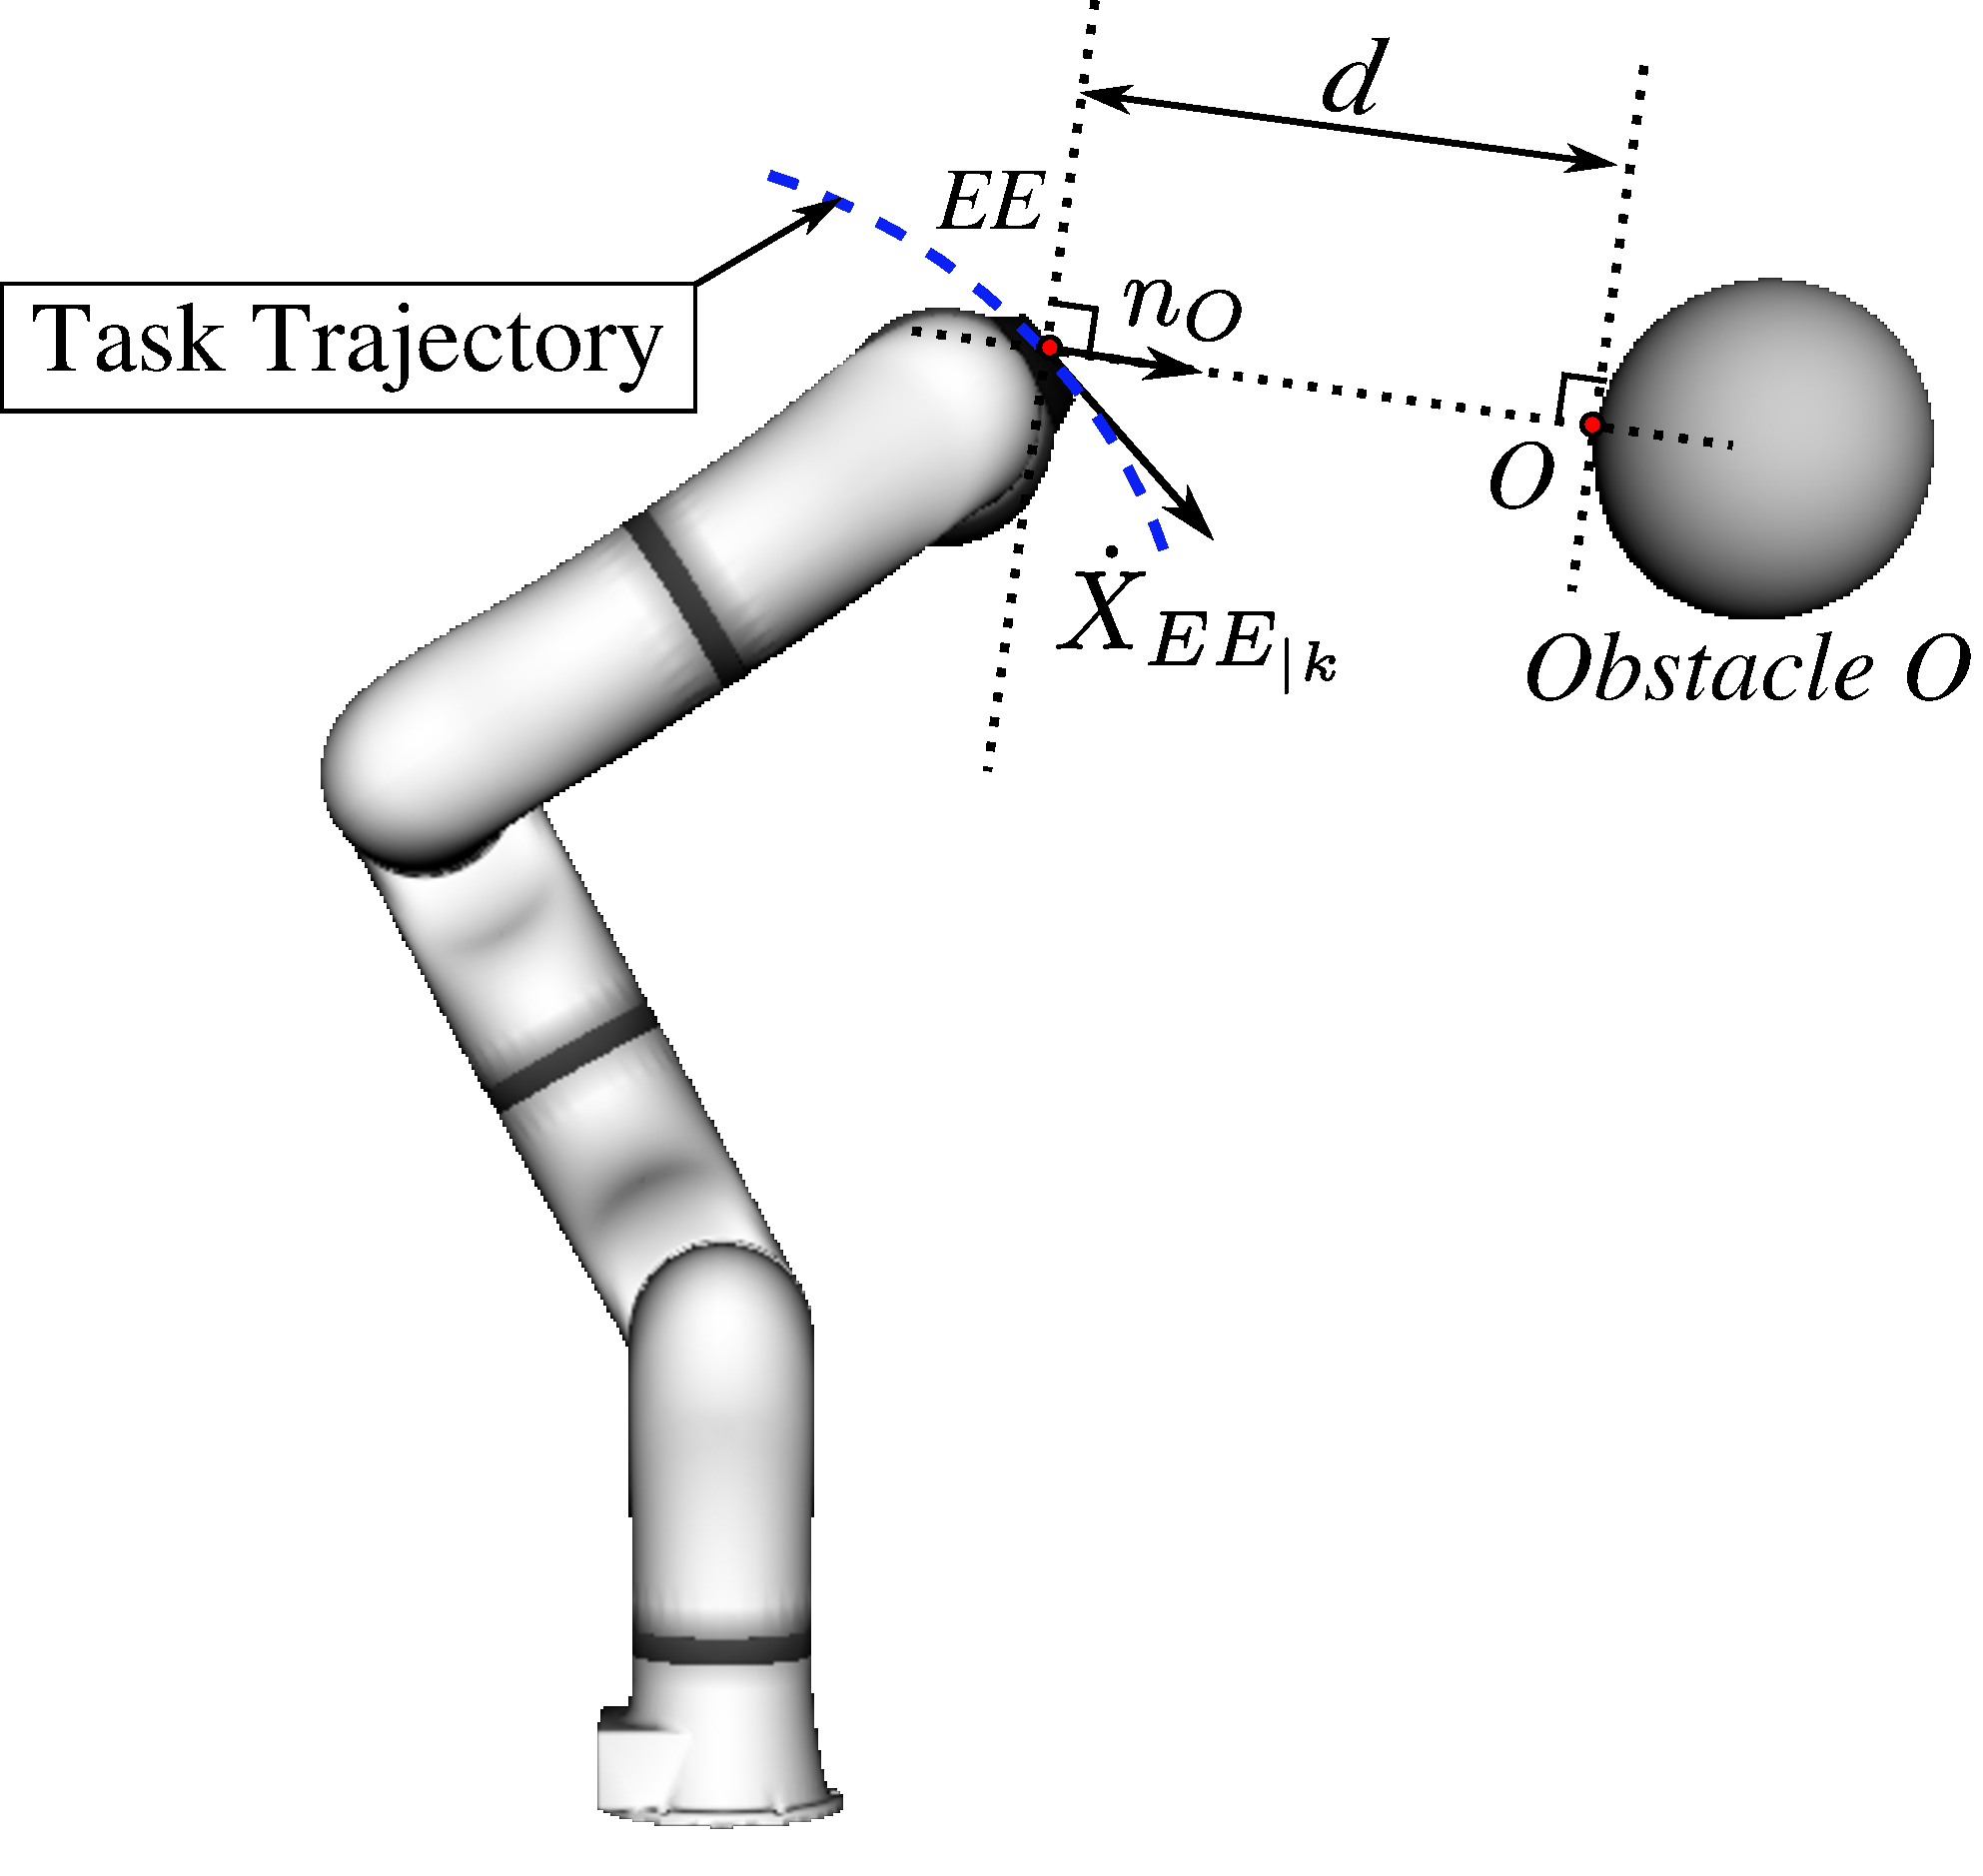
\includegraphics[width=0.5\linewidth]{\figurepath/obstacle_nobackground.pdf}
\caption{Description of the obstacle avoidance constraint.}
\label{fig:scenario obstacle}
\end{figure}
As shown in Figure \ref{fig:scenario obstacle}, the obstacle avoidance constraint can be defined as requiring the minimum distance $d=\| \vect{x}_{r\vert k}-\vect{x}_{o\vert k}\|$ between the robot body and the obstacle to be positive. Using a discrete linear approximation with a time step of $\delta t$, the minimum distance $d_{k+1}$ can be expressed as
\begin{singlespace}
\begin{equation}\label{eq:obstacle constraint original}
d_{k+1} = d_{k} + \vect{n}^T(\vect{\dot{x}}_{r\vert k}-\vect{\dot{x}}_{o\vert k})\delta t + \frac{\delta t^2}{2}\vect{n}^T (\vect{\ddot{x}}_{r\vert k}-\vect{\ddot{x}}_{o\vert k}) ~,
\end{equation}
\end{singlespace}
\noindent where $\vect{n}$ is the vector associated to the shortest distance segment from the robot to the object, $\vect{x}_{r\vert k}$ and $\vect{\dot{x}}_{r\vert k}$ are the current position and velocity of the robot, $\vect{\ddot{x}}_{r\vert k}$ is the acceleration resulting from the next control action. It is worth noting that constraint \eqref{eq:obstacle constraint original} relies on the knowledge of  $\vect{x}_{o\vert k}, \vect{\dot{x}}_{o\vert k}$ and $\vect{\ddot{x}}_{o\vert k}$, which are the current position, velocity and acceleration of the obstacle. If the velocity and acceleration of the obstacle are not known, \textit{i.e.} measured or estimated, \eqref{eq:obstacle constraint original} assumes that the obstacle is static over a control period, which can be a valid working assumption. Using the kinematic relationship between the operational space velocity/acceleration and the generalized coordinates, \eqref{eq:obstacle constraint original} can be expressed linearly with respect to $\vect{\ddot{q}}_k$ as
\begin{singlespace}
\begin{equation}\label{eq:obstacle constraint}
\begin{split}
d_{k}  + \vect{n}^T(J(\vect{q}_k)\vect{\dot{q}}_k-\vect{\dot{x}}_{o\vert k})\delta t
+ \frac{\delta t^2}{2}\vect{n}^T(J(\vect{q}_k)\vect{\ddot{q}}_{k}+\dot{J}(\vect{q}_k)\vect{\dot{q}}_k-\vect{\ddot{x}}_{o\vert k})\geq 0 ~.
\end{split}
\end{equation}
\end{singlespace}


\subsubsection{Contact Constraints}
For a single point in rigid contact, there are two constraints to be respected in order to maintain a non-sliding contact between two objects. One is contact existing constraint, and the other is friction cone constraint.

(1) \textbf{Contact existing constraint:} Contact existing constraint is prerequisite to maintain a contact, which includes the kinematics condition and force condition. Kinematics condition means that there is no relative movement between two objects. Assuming that the environment is static and rigid, the contact is maintained only if the velocity of the robot contact body are zero: $\vect{\ddot{x}}_c = 0$. This condition can be expressed in terms of joint accelerations:
\begin{singlespace}
\begin{equation}
\vect{\ddot{x}}_c=\mathbf{J}_c(\vect{q})\vect{\ddot{q}} + \mathbf{\dot{J}}_c(\vect{q},\vect{\dot{q}})\vect{\dot{q}}=0 ~, \label{eq:cons zero velocity}\\
\end{equation}
\end{singlespace}
\noindent At each contact point, contact force condition is a supplementary for kinematics condition. The contact force along the normal direction is nonnegative. This means that either the robot pushes against the environment without movement, or the robot does not apply a force on the environment.
\begin{singlespace}
\begin{equation}
F_n  \geq 0 ~. \label{eq:cons nonnegative force}
\end{equation}
\end{singlespace}
\noindent These two conditions constitute the contact existing constraint, which can sufficiently maintain a rigid contact between the robot body and the environment.

(2) \textbf{Friction cone constraint:} To ensure a non-sliding contact, the contact force for each contact point is constrained within the Coulomb friction cone: $\left\|\vect{F}_t\right\|  \leq \mu  \left\|\vect{F}_n \right\|$, where $\mu$ is the friction coefficient. The friction cone is usually approximated by a polygonal cone so that the non-sliding contact constraint can be expressed as a set of linear inequality constraints \cite{siciliano2008}: 
\begin{singlespace}
\begin{equation}\label{eq:cons friction cone}
C \vect{F}_c \leq 0 ~.
\end{equation}
\end{singlespace}


\subsection{Quadratic Program Control Scheme}
This thesis deals with multiple tasks subject to multiple constraints. This multi-objective control problem can be formulated as a Linear Quadratic Programming problem (LQP) \cite{salini2011}. The action variable $\vect{\chi}^*$ is resolved in one LQP by minimizing a cost function associated with a set of tasks $\vect{e}(\vect{\chi})$, while satisfying equality constraints like the equation of motion \eqref{eq:dynamic model} and zero velocity at contact point \eqref{eq:cons zero velocity}, and inequality constraints,such as joint limits and actuation capacities \eqref{eq:limit q}-\eqref{eq:limit tau}, obstacle avoidance constraint \eqref{eq:obstacle constraint}, and contact constraints \eqref{eq:cons nonnegative force}-\eqref{eq:cons friction cone}. Based on weighting strategy \cite{collette2007, liu2012}, the control problem can be formulated in a generic form as:
\begin{singlespace}
\begin{equation}\label{eq:lqp}
    \begin{array}{cc}
     \argmin \limits_{\vect{\chi}} & \sum\limits_{i=1}^{n_{t}} (\left \| \vect{e}_i(\vect{\ddot{q}}) \right \|^2_{\mathbf{Q}_i}) + \left \| \vect{\chi} \right \|^2_{\mathbf{Q}_r} \\
       \text{subject to} & \eqref{eq:eq cons}~~ \& ~~\eqref{eq:ineq cons}
    \end{array}
    ~.
\end{equation}
\end{singlespace}

The notation $\left \| \vect{a} \right \|^2_Q$ is the shorthand of the form $\vect{a}^T Q \vect{a}$. $\mathbf{Q}_i=\omega_i \mathbf{I}_{m_i}$ is a weighting matrix to regulate the importance level of task $i$, with $\omega_i$ denoting the weight of task objective $i$. $\mathbf{Q}_r=\omega_r \mathbf{I}_{n+n_a+3n_c}$ is the weighting matrix of the regularization term, with $\omega_r$ denoting the weight value. The regulation term minimizes the norm of joint accelerations and the action variable. For a redundant robot with many solutions satisfying the same task objective, the regulation term is useful for ensuring the uniqueness of the solution. As the regulation term may increase task error, $\omega_r$ is usually a very small compared to $\omega_i$. By solving \eqref{eq:lqp}, the action variable $\vect{\chi}$ can be obtained, from which the solution of actuation torques $\vect{\tau}$ is extracted to actuate the robot.



%\begin{singlespace}
\begin{subequations}\label{eq:ghc}
\begin{eqnarray}
\mathop{{\arg\min}\vphantom{\sim}}\limits_{\substack{\ddot{\vect{q}}^{\prime},\vect{\chi}}}
& \sum\limits_{i=1}^{n_{t}} \left\Vert  \vect{e}_{i}\left(\ddot{\vect{q}}_{i}^{{\prime}} \right) \right\Vert^2 
+ \left\Vert \left[\begin{array}{c} \ddot{\vect{q}}^{\prime}\\ \vect{\chi} \end{array}\right] \right\Vert_{\mathbf{Q}_r}^2\label{eq:ghc obj}\\  
 \text{subject to} 
        & \mathbf{A}(\vect{q, \dot{q}})\left(\begin{array}{c} \vect{\ddot{q}} \\ \vect{\chi} \end{array} \right) = \vect{b}(\vect{q, \dot{q}})  \label{eq:ghc eq cons}\\ 
        & \mathbf{G}(\vect{q, \dot{q}})\left( \begin{array}{c} \vect{\ddot{q}} \\ \vect{\chi} \end{array} \right) \leq \vect{h}(\vect{q, \dot{q}}) \label{eq:ghc ineq cons} \\
        &\ddot{\vect{q}} = \mathbf{P}\ddot{\vect{q}}^{\prime} =\sum_{i=1}^{n_{t}} \mathbf{P}_{i}(\mathbf{W}_i) \ddot{\vect{q}}_{i}^{{\prime}} \label{eq:ghc ddq}
\end{eqnarray}                
\end{subequations}
\end{singlespace}


\textbf{Chapter 5}
\begin{synopsis}
	Based on the control framework proposed in the Section \ref{sec:force control framework}, Model Predictive Control works as a high-level controller to generate a continuous obstacle avoidance constraint in order to minimize sudden changes in joint torques caused by moving obstacle in this chapter. The MPC previews the position of the moving obstacle in time and generates continuous position, velocity and acceleration profiles of the obstacle. Furthermore, a continuous obstacle avoidance constraint can be obtained. Section \ref{sec:motion intro} reviews techniques to deal with  obstacle avoidance for robots. Section \ref{sec:motion constraint} proposes a new obstacle avoidance constraint including position, velocity and acceleration profiles of the obstacle, which are used to generate continuous obstacle avoidance constraint using MPC. A sensitive analysis is carried out to find the effects of the parameters of the MPC. To illustrate the effectiveness of the proposed approach, Section \ref{sec:motion results} shows the simulation results on the Kuka LWR robot and the iCub robot in different scenarios. Section \ref{sec:motion conclusion} concludes the chapter by summarizing the contributions.  
\end{synopsis}

%=========================================================================

\section{Introduction}
\label{sec:motion intro}
Robot collision avoidance is traditionally treated as a planning problem, and research in this area has focused on the development of collision-free path planning algorithm \cite{gouzenes1984,lumelsky1987,hsu2002,gonzalez2006}. These algorithms provide a path that will enable the robot to accomplish its assigned task free from any risk of collisions. The advantage of the planning approach is that it can obtain a global solution. However, the robot is limited to the execution of elementary operations for which the paths have been precisely specified. Additionally, global trajectory planning is not only a time-consuming technique, but also incapable of dealing with trajectory replanning due to changing situations. Therefore, using planning algorithms to avoid collisions is not sufficient if robots are operating in an unstructured and dynamic environment.

A complementary way to achieve real-time obstacle avoidance is to integrate environment sensing feedback to the reactive controller . The advantage of reactive obstacle avoidance is to compute control actions by introducing the sensor information within the control loop. The artificial potential filed (APF) approach in \cite{khatib1986} is a well-established approach to deal with obstacle avoidance. The created virtual field around the obstacle induces repulsive forces applied on the robot when it gets too close to the obstacle. These potential fields are built around the obstacle and allow real-time reactive control. The Gradient Projection Method (GPM) \cite{liegeois1977} has been widely used in the literature by utilizing the null-space projector to deal with inequality constraints. Based on this framework, a low-level controller is proposed with two components in \cite{maciejewski1985, brock2002}: the principal goal is the desired task and the secondary is the obstacle avoidance projected into the null-space of the task. Herein, obstacle avoidance is realized in the null-space of the task objective. It is given a higher priority if that null-space is not sufficient to ensure collision-free motion. The same idea is applied in \cite{stasse2008,sugiura2010,dietrich2012b} to handle self-collision avoidance in a task hierarchy using the null-space projector. However, obstacle avoidance is treated as tasks in these analytical methods. Once the controller has to cope with other inequality constraints, the analytical methods becomes more complex and is not easy to be solved.

Quadratic Programming provides a mathematical framework particularly suitable to the formulation of the controller while accounting for tasks and constraints simultaneously. It allows to explicitly write the control problem as objectives to be reached under a certain set of constraints.  In \cite{faverjon1987, zhang2004obstacle}, a Quadratic Programming control structure is proposed to handle obstacle avoidances. In this controller, obstacle avoidances are treated as inequality constraints, which limit the robot's velocities toward obstacle. The work in \cite{salini2012} integrates the position, velocity and acceleration of both the robot and obstacle to the obstacle avoidance constraint. The constraint with dynamic parameters of the system is created to keep the minimum distance between the robot and the obstacle positive.

All these solutions are adapted to local procedures and cannot be applied in more complex context, for example when robots have to reach some goals in highly cluttered spaces. Additionally, these approaches neglect one important case of the obstacle moving rapidly in the dynamic environment. When the obstacle moves rapidly, the obstacle avoidance constraint stated above will be discontinuous and result in large changes in actuator torques when solving the control problem. To solve this problem, a new obstacle avoidance constraint is formulated and a Model Predictive Control scheme is employed. The MPC is used to preview movements of the obstacle and generate a new obstacle avoidance constraint that result in minimized changes in actuator torques.

\section{Motion constraint generation}
\label{sec:motion constraint}

Due to the rapid movements of the obstacle, large instantaneous changes of $h_i$ in \eqref{eq:cp ineq cons} can result in large instantaneous changes joint torques when solving the control problem as stated in Section \ref{sec:Problem statement}. In order to prevent large instantaneous changes in joint torques, an intuitive method is to minimize changes of the obstacle avoidance constraint when a rapid movements occurs. In this section, an approach using MPC is proposed to preview movements of the obstacle and generate a continuous obstacle avoidance constraint.

\subsection{Obstacle avoidance constraint}
\label{sec:motion obstacle constraint}
\begin{figure}[!h]
\centering
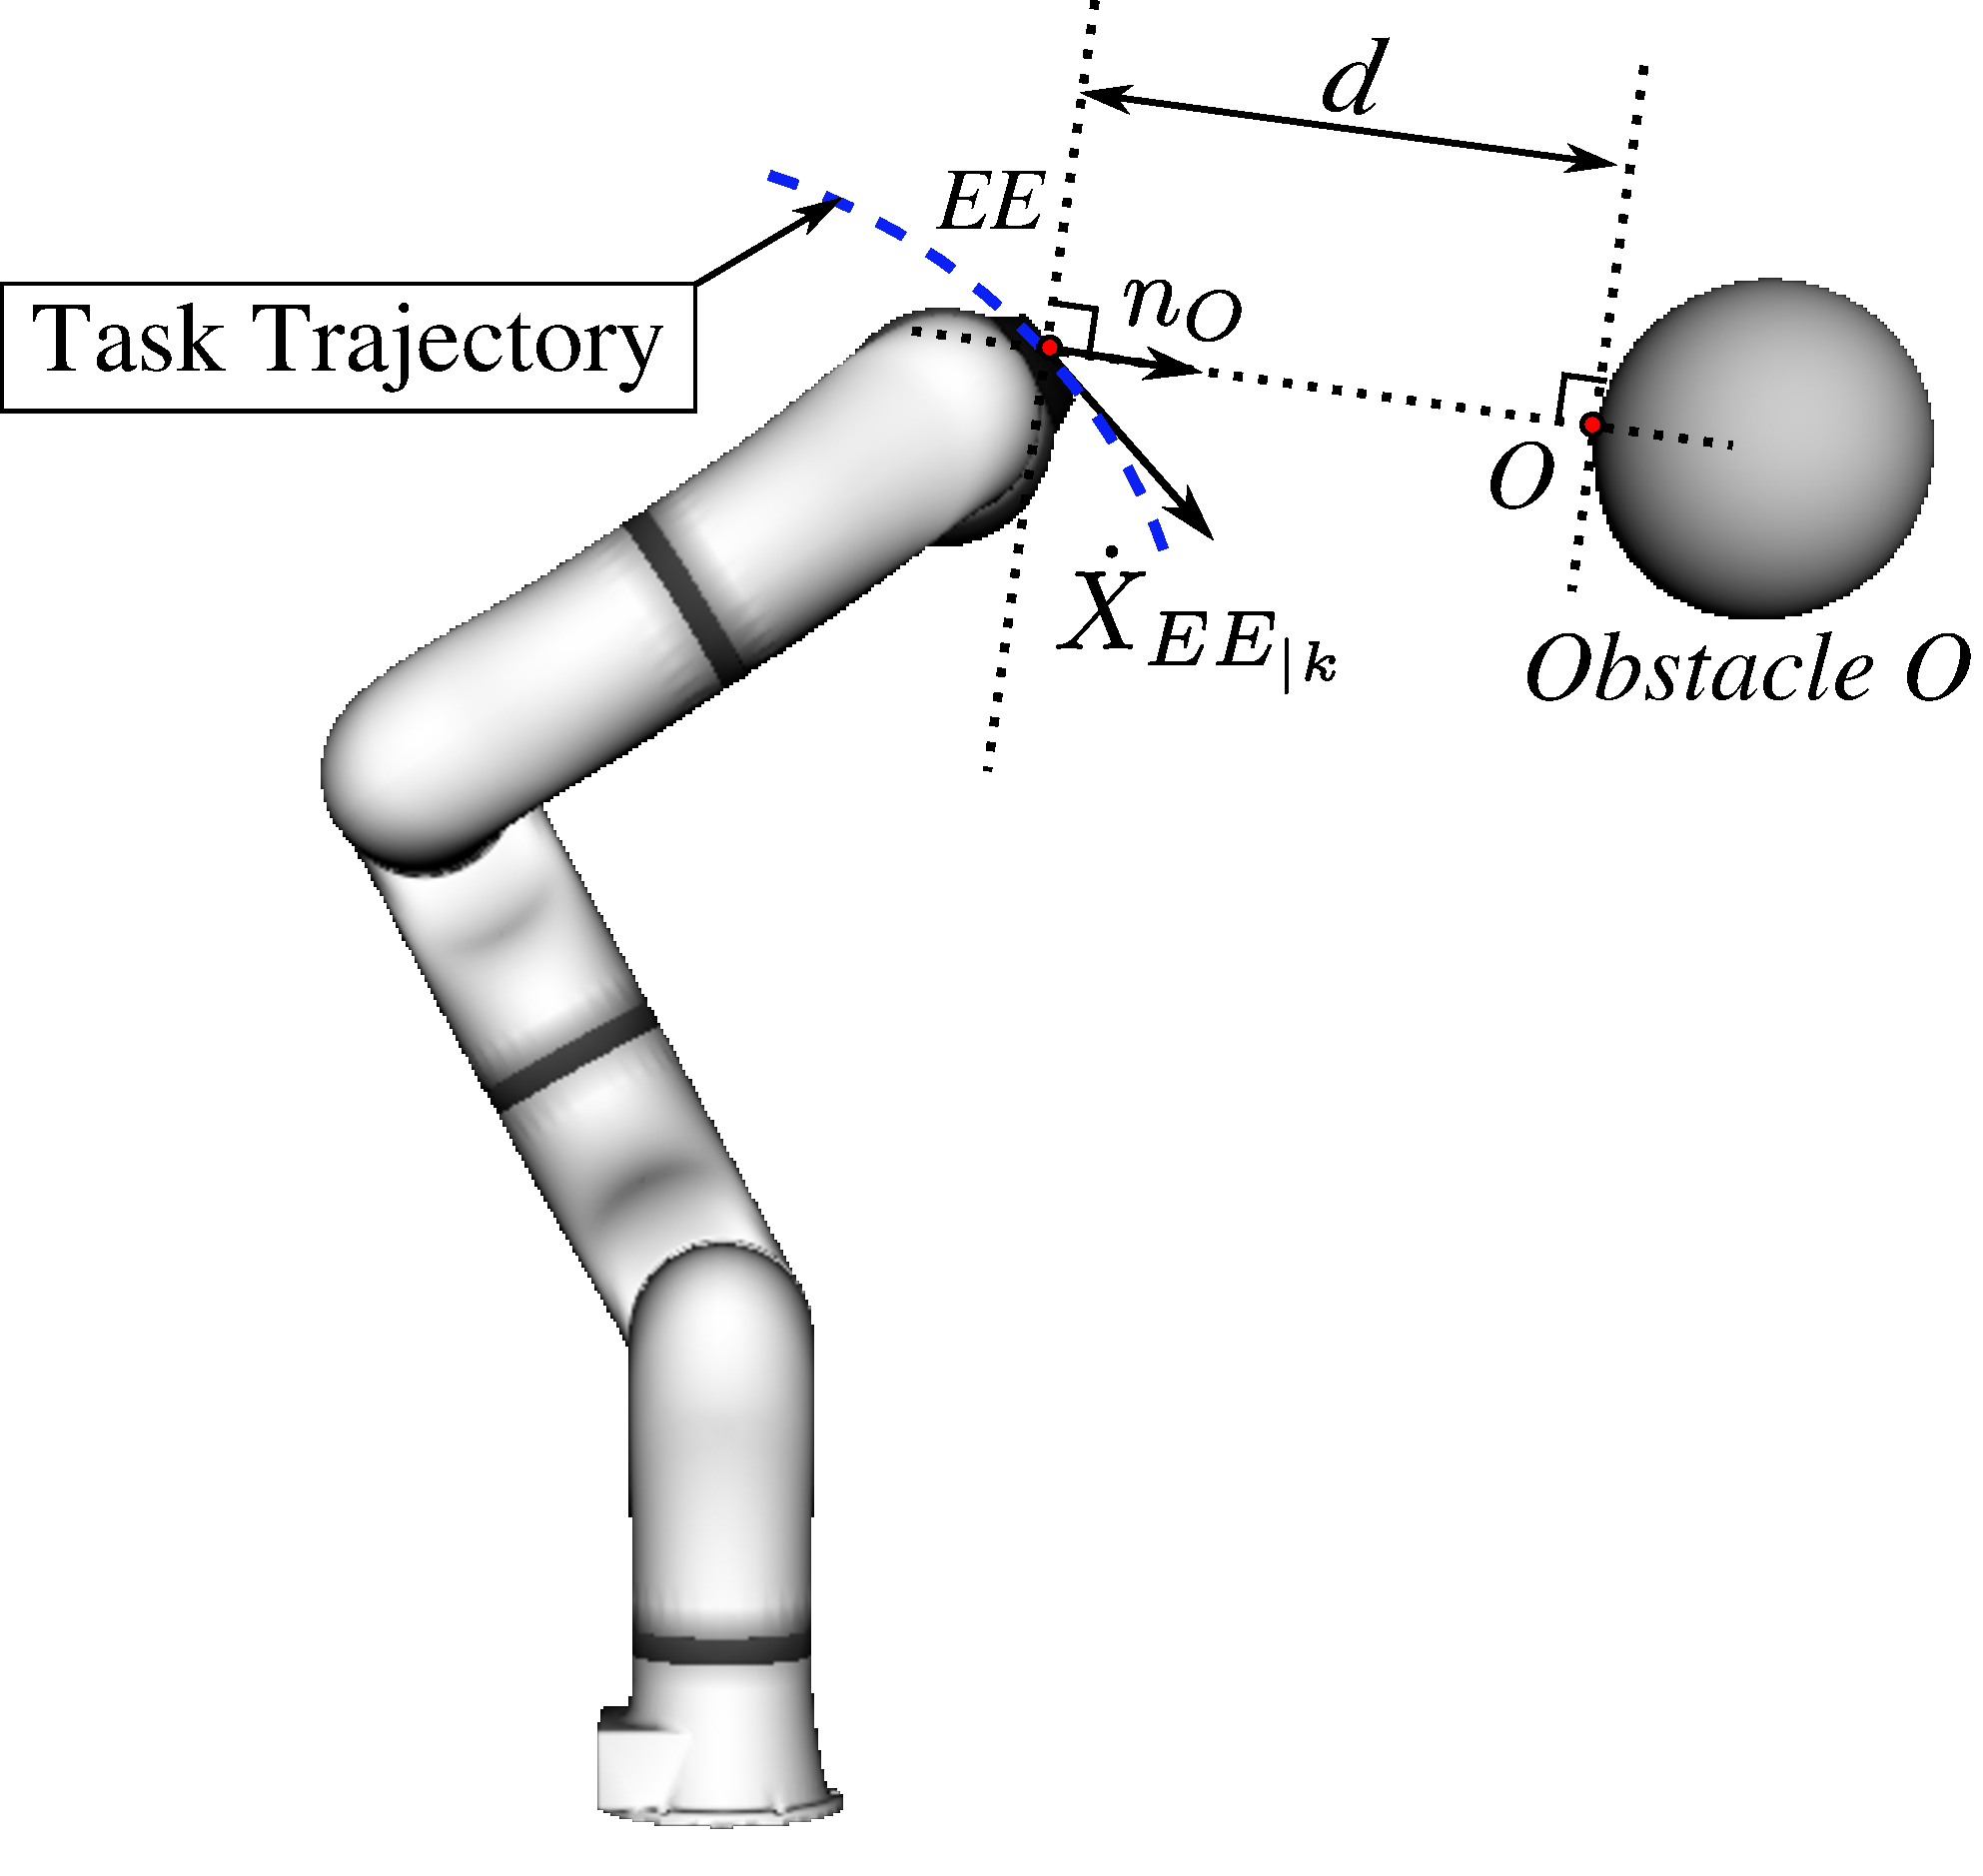
\includegraphics[width=0.4\linewidth]{\figurepath/obstacle_nobackground.pdf}
\caption{Description of the obstacle avoidance constraint.}
\label{fig:obstacle}
\end{figure}
To prevent any collision, the obstacle avoidance constraint can be defined as requiring the minimum distance $d=\| \vect{p}_{r,~k}-\vect{p}_{o,~k}\|$ between the robot body and the obstacle to be strictly non-zero \cite{faverjon1987, kanehiro2008}, where $\vect{p}_{\bullet,~k}=\left[x_{\bullet,~k}~y_{\bullet,~k}~z_{\bullet,~k}\right]^T$ represents the position in Cartesian space at time $k$. Using a discrete linear approximation with a time step of $\delta t$, the minimum distance $d_{k+1}$ can be expressed as:
\begin{singlespace}
\begin{equation}\label{eq:obstacle constraint original}
d_{k+1} = d_{k} + \vect{n}_o^T(\vect{\dot{p}}_{r,~k}-\vect{\dot{p}}_{o,~k})\delta t + \frac{\delta t^2}{2}\vect{n}_o^T (\vect{\ddot{p}}_{r,~k}-\vect{\ddot{p}}_{o,~k}) ~,
\end{equation}
\end{singlespace}

\noindent where $\vect{n}_o$ is the vector associated to the shortest distance from the robot to the object. The vector $\vect{n}_o$ is assumed to evolve continuously in this paper. $\vect{p}_{r,~k}$ and $\vect{\dot{p}}_{r,~k}$ are the current position and velocity of the robot, $\vect{\ddot{p}}_{r,~k}$ is the acceleration resulting from the next control action. They evolves continuously according to the continuous motion task or force task. It is worth noting that constraint \eqref{eq:obstacle constraint original} relies on the knowledge of  $\vect{p}_{o,~k}, \vect{\dot{p}}_{o,~k}$ and $\vect{\ddot{p}}_{o,~k}$ which are the current position, velocity and acceleration of the obstacle. If the velocity and acceleration of the obstacle are unknown, \textit{i.e.} neither measured nor estimated, \eqref{eq:obstacle constraint original} assumes that the obstacle is quasi-static over a control period which can be a valid working assumption. Using the kinematic relationship between the operational space velocity/acceleration and the generalized coordinates in \eqref{eq:obstacle constraint original}, the obstacle avoidance constraint can be expressed linearly with respect to $\vect{\ddot{q}}_k$ as:
\begin{singlespace}
\begin{equation}\label{eq:obstacle constraint}
\begin{split}
& d_{k}  + \vect{n}_o^T(J(\vect{q}_k)\vect{\dot{q}}_k-\vect{\dot{p}}_{o,~k})\delta t+\frac{\delta t^2}{2}\vect{n}_o^T(J(\vect{q}_k)\vect{\ddot{q}}_{k}+\dot{J}(\vect{q}_k)\vect{\dot{q}}_k-\vect{\ddot{p}}_{o,~k})\geq 0 \\
\Leftrightarrow & -J(\vect{q}_k)\vect{\ddot{q}}_{k} \leq d_{k}  + \vect{n}_o^T(J(\vect{q}_k)\vect{\dot{q}}_k-\vect{\dot{p}}_{o,~k})\delta t+\frac{\delta t^2}{2}\vect{n}_o^T(\dot{J}(\vect{q}_k)\vect{\dot{q}}_k-\vect{\ddot{p}}_{o,~k}) 
\end{split}~.
\end{equation}
\end{singlespace}

\subsection{Motion constraint generation}
According to the obstacle avoidance constraint \eqref{eq:obstacle constraint}, $h_i$ can be expressed as:
\begin{singlespace}
\begin{equation}\label{eq:obstacle constraint h_i}
h_i=d_{k}(\vect{p}_{r},\vect{p}_{o})+\vect{n}_o^T(J(\vect{q})\vect{\dot{q}}-\vect{\dot{p}}_{o})\delta t +\frac{\delta t^2}{2}\vect{n}_o^T(\dot{J}(\vect{q})\vect{\dot{q}}-\vect{\ddot{p}}_{o}) ~.
\end{equation}  
\end{singlespace}

\noindent $h_i$ is a function of the position, velocity and acceleration of the obstacle. In fact the movement of the obstacle along any axis in Cartesian space is independent. Without loss of generality, the position, velocity and acceleration along the $x-$axis for instance are formulated in the following part of this thesis. In this case, a linear discrete-time dynamic model of the obstacle can be created in state space form:
\begin{singlespace}
\begin{equation}\label{eq:state space form}
\underbrace{\left[\begin{array}{c} x_{o,~k+1} \\ \dot{x}_{o,~k+1} \\ \ddot{x}_{o,~k+1}\end{array}\right]}_{\vect{X}_{o,~k+1}}  = \underbrace{\left[\begin{array}{ccc} 1 & T & T^2/2 \\ 0 & 1 & T \\ 0 & 0 & 1 \end{array} \right]}_{\mathbf{A}} \underbrace{\left[\begin{array}{c} x_{o,~k} \\ \dot{x}_{o,~k} \\ \ddot{x}_{o,~k}\end{array}\right]}_{\vect{X}_{o,~k}} + \underbrace{\left[\begin{array}{c} T^3/6 \\ T^2/2 \\ T \end{array} \right]}_{\mathbf{B}} \dddot{x}_{o,~k} ~,
\end{equation}
\end{singlespace}

\noindent where $\vect{X}_{o,~k}$ and $\dddot{x}_{o,k}$ are the state vector of the obstacle and the control action at time $k$, respectively. Matrices $\mathbf{A}$ and $\mathbf{B}$ implicitly describe the linearity of the system.
%\begin{equation*}
%\begin{array}{cc}
%A = \left[\begin{array}{ccc} 1 & T & T^2/2 \\ 0 & 1 & T \\ 0 & 0 & 1 \end{array} \right], &
%B = \left[\begin{array}{c} T^3/6 \\ T^2/2 \\ T \end{array} \right].
%\end{array}
%\end{equation*}
 
Using the dynamic model \eqref{eq:state space form} recursively, at time $k$, the relationships between the control action vector and state vectors over a finite time horizon $NT$ is given by:
\begin{singlespace}
\begin{equation}\label{eq:state space form N horizon}
\hat{\vect{X}}_o =\hat{\mathbf{A}}\vect{X}_{o,~k}+\hat{\mathbf{B}}\vect{U}_o ~,
\end{equation}
\end{singlespace}

\noindent where,
\begin{singlespace}
\begin{equation*}
\begin{array}{cc}
\hat{\vect{X}}_o = \left[\begin{array}{c} \vect{X}_{o,~k+1\vert k} \\ \vect{X}_{o,~k+2\vert k} \\ \vdots \\ \vect{X}_{o,~k+N\vert k} \end{array} \right], &
\hat{\mathbf{A}} = \left[\begin{array}{c} \mathbf{A} \\ \mathbf{A}^2 \\ \vdots \\ \mathbf{A}^N \end{array} \right],
\end{array}
\end{equation*}
\end{singlespace}


\begin{singlespace}
\begin{equation*}
\begin{array}{cc}
\hat{\mathbf{B}} = \left[\begin{array}{cccc} \mathbf{B} & 0 & \cdots & 0 \\
\mathbf{A}\mathbf{B} & \mathbf{B} & \cdots & 0 \\ \vdots & \vdots & \ddots & \vdots \\ \mathbf{A}^{N-1}\mathbf{B} & \mathbf{A}^{N-2}\mathbf{B} & \cdots & \mathbf{B} \end{array} \right], &
\vect{U}_o =  \left[\begin{array}{c} \dddot{x}_{o,~k\vert k} \\ \dddot{x}_{o,~k+1\vert k} \\ \vdots \\ \dddot{x}_{o,~k+N-1\vert k} \end{array} \right].
\end{array}
\end{equation*}
\end{singlespace}


%Given the measured or predicted location of the obstacle $\vect{x}_o^{m}=\left[ x_{o,x}^m ~~ x_{o,y}^m ~~ x_{o,z}^m  \right]^T$ over a time window\footnote{Based on sensors and/or the control scenario, see Figure~\ref{fig:block diagram}.}, a continuous evolution of $\vect{x}_o^*,\vect{\dot{x}}_o^*,\vect{\ddot{x}}_o^*$ can be calculated to generate a continuous $h_i^*$.


Over the time horizon, the position of the obstacle may be measured by scenarios in advance, which is $\vect{x}^{m}_{o}=\left[x_{o,~k+1}^{m}~\dots~x_{o,~k+N}^{m}\right]^T$. In order to take advantage of $\vect{x}^{m}_{o}$, the predicted positions over the preview horizon can be extracted from $\hat{\vect{X}}_o$: $\hat{\vect{X}}_{o,~x}=\left[x_{o,~k+1\vert k}~\dots~x_{o,~k+N\vert k}\right]^T$. According to \eqref{eq:state space form N horizon}, $\hat{\mathbf{A}}_x$ and $\hat{\mathbf{B}}_x$ can be derived from $\hat{\mathbf{A}}$ and $\hat{\mathbf{B}}$, respectively. Therefore, the predicted position of the obstacle over the horizon can be formulated as:
\begin{singlespace}
\begin{equation}
\hat{\vect{X}}_{o,~x} =\hat{\mathbf{A}}_x\vect{X}_{o,~k}+\hat{\mathbf{B}}_x\vect{U}_o ~.
\end{equation}
\end{singlespace}

\noindent To approximate the movement of the obstacle using measured position information $\vect{x}_o^m$, the optimization problem of the MPC is formulated similarly to \eqref{eq:mpc force}:

\begin{singlespace}
\begin{subnumcases}{\label{eq:mpc motion} \dddot{x}_{o,~k\vert k}^*=}
  \argmin \limits_{\vect{U}_o} & $\left\|\hat{\vect{X}}_{o,~x}-\vect{x}^{m}_{o}\right\|^2+\beta\|\vect{U}_o \|^2$ \label{eq:mpc motion obj}\\
       \text{subject to} & $\hat{\vect{X}}_{o,~x} =\hat{\mathbf{A}}_x\vect{X}_{o,~k}+\hat{\mathbf{B}}_x\vect{U}_o$\label{eq:mpc motion model}\\ 
       \phantom{1}       & $\hat{\vect{X}}_{o,~x} \geq \vect{x}^{m}_{o}$ \label{eq:mpc motion ineq} \\
\end{subnumcases} 
\end{singlespace}



Then, at time $k$, $\dddot{x}_{o,~k\vert k}^*$ can be calculated by a QP solver and it is used to update $\vect{X}_{o,~k+1}^*= \mathbf{A} \vect{X}_{o,~k}^* + \mathbf{B} \dddot{x}_{o,~k\vert k}^*$. Therefore, continuous evolution of $\vect{X}_o^* = \left[ \vect{x}_o^*~ \vect{\dot{x}}_o^*~\vect{\ddot{x}}_o^* \right]^T$ can be generated (similarly for $\vect{Y}_{o}^*$ and $\vect{Z}_{o}^*$). $\vect{p}_o$, $\vect{\dot{p}}_o$ and $\vect{\ddot{p}}_o$ are thus continuous. Based on \eqref{eq:obstacle constraint h_i} continuous $h_i^*$ can be obtained.

\begin{figure}[!htb]
\centering
\subfigure[Evolution of $\vect{x}_o^m$ and $\vect{x}_o^*$.]
{\includegraphics[width=0.31\linewidth]{\figurepath/d05_N15_R5_pos.pdf}} \quad
\subfigure[Evolution of $\vect{\dot{x}}_o^*$ and $\vect{\ddot{x}}_o^*$.]
{\includegraphics[width=0.29\linewidth]{\figurepath/d05_N15_R5_va.pdf}} \quad
\subfigure[Evolution of $\vect{\dddot{x}}_o^*$.]
{\includegraphics[width=0.31\linewidth]{\figurepath/d05_N15_R5_jerk.pdf}}\quad
\caption{The optimized constraint with $T=0.01s$, $NT=1.0s$ and $\beta=10^{-5}$.}
\label{fig:MPC constant ratio}
\end{figure}


To illustrate this concept, a simple example is provided to handle the discontinuities in $\vect{x}^{m}_{o}$. MPC \eqref{eq:mpc motion} is used with time step $T = 0.01s$, constant ratio $\beta=10^{-5}$ and time horizon $NT=1.5s$. In Figure \ref{fig:MPC constant ratio}(a), the generated $\vect{x}_{o}^*$ is continuous compared with the original position $\vect{x}^{m}_{o}$. Moreover, MPC also generates continuous $\vect{\dot{x}}_o^*$ and $\vect{\dot{x}}_o^*$ in Figure \ref{fig:MPC constant ratio} and continuous $\vect{\dddot{x}}_{o}^*$ in Figure \ref{fig:MPC constant ratio}(b). With the weight $\beta=10^{-5}$, MPC minimizes the error between the solution of $\vect{x}_o^*$ and the original position $\vect{x}_o^m$ as well as reduces the instantaneous variation of $\vect{\dddot{x}}_{o}$. However, there exist overshoots at $t=4.0s$ and $t=6.0s$. These overshoots are mainly due to a relatively small weight $\beta$ of the regulation term $\|\vect{U}_o \|^2$. Additionally, the preview horizon $NT$ also affects the variations of $\vect{\dddot{x}}_o$. Therefore, the influences of the weight $\beta$ and the prediction horizon $NT$ on the variations of $\vect{\dddot{x}}_o$ are analysed in the following section. 
%which reduces the instantaneous variation of $\vect{\dddot{x}}_o$, with respect to $\left\|\hat{\vect{X}}_{o,~x}-\vect{x}^{m}_{o}\right\|^2$, which minimizes the distance to the original reference. Large variations of $\vect{\dddot{x}}_o$ is the real cause for overshoots. Moreover, 


\subsection{Analysis on the parameters of MPC for motion}
The example in Figure \ref{fig:MPC constant ratio} illustrates that the proposed approach \eqref{eq:mpc motion} can generate continuous evolution of $\vect{x}_o^*$, $\vect{\dot{x}}_o^*$ and $\vect{\ddot{x}}_o^*$ with respect to a discontinuous evolution of the obstacle position $\vect{x}^{m}_{o}$. Large variation of $\vect{\dddot{x}}_o$ can cause overshoots at the instant when $\vect{x}_o^m$ changes largely. Based on \eqref{eq:mpc motion}, the maximal jerk $\vect{\dddot{x}}_o$ is affected by the weight $\beta$ and the prediction horizon $NT$. In order to effectively minimize the maximum jerk and avoid overshoots, the weight $\beta$ and the prediction horizon $NT$ should be optimized. The criteria for choosing $\beta$ and $NT$ is analysed and summarized in this section.

\subsubsection{The weight}

\begin{figure}[!h]
\centering
\includegraphics[width=0.8\linewidth]{\figurepath/d05_N10.pdf}
\caption{Evolution of $x_o^*$ and $x_o^m$ using a set of different $\beta$s with the prediction horizon $NT=1.0s$.}
\label{fig:weight analysis}
\end{figure}

The weight $\beta$ regulates the importance between the regulation term $\left\|\vect{U}_o \right\|^2$ and the approximation term $\left\|\hat{\vect{X}}_{o,~x}-\vect{x}^{m}_{o}\right\|^2$ in \eqref{eq:mpc motion}. Since the weight for the approximation term is $1$, a relatively large weight $\beta$ means that the maximum jerk $\vect{\dddot{x}}_o$ is reduced. Given the prediction horizon $NT=1.0s$, $x_o^m$ suddenly changes at $t_1=4.0s$ and the MPC can preview this change at $t=3.0s$. The results generated by the MPC using a set of different $\beta$s are shown in Figure \ref{fig:weight analysis}. Although the weight $\beta$ increases from $10^{-8}$ to $10^{-1}$, the overshoots still exist. Indeed, the generated $x_o^*$ oscillates when $\beta$ is $10^{-1}$. A relatively larger weight $\beta$ cannot ensure a better results rather than oscillations. Therefore, it is impossible to avoid overshoots only by modifying the weight $\beta$. 

\subsubsection{The length of the horizon window}

\begin{figure}[!h]
\centering
\includegraphics[width=0.8\linewidth]{\figurepath/d05_R5.pdf}
\caption{Evolution of $x_o^*$ and $x_o^m$ using a set of different $NT$s with the weight $\beta=10^{-5}s$.}
\label{fig:horizon analysis}
\end{figure}

The prediction horizon $NT$ enables the MPC to react to future changes accordingly. Given the weight $\beta=10^{-5}$, Figure \ref{fig:horizon analysis} shows the generated smooth evolution $x_o^*$ with respect to the discontinuous $x_o^m$ with a set of different $NT$s using the MPC. The magnitude of the overshoot at $t_1=4.0s$ decreases as the prediction horizon increases from $NT=0.3s$ to $NT=0.9s$. Then although the prediction horizon continues to increase from $NT=0.9s$ to $NT=3.0s$, the magnitude of the overshoot just decreases very little and the overshoots are not eliminated. Therefore, the overshoots of $x_o^m$ cannot be avoided only by extending the prediction horizon $NT$.

In summary, the overshoots cannot be removed by tuning the weight $\beta$ and the prediction horizon $NT$. It is necessary to find a way to deal with this problem when solving the MPC problem \eqref{eq:mpc motion}.

\subsubsection{Dynamic weighting matrix}
Through the analysis on the weight $\beta$ and the prediction horizon $NT$, it is observed that the weight plays a more important role in the generated results than the prediction horizon. The weight strictly guarantees the approximation to the original position. Given a constant weight, the steady increase of prediction horizon cannot enable the MPC to eliminate the overshoots, but increase the computation cost. The constant weight $\beta$ limits the potential of the prediction horizon. In order to reduce the magnitude of the overshoots or even eliminate the overshoots, a dynamic weighting matrix $\mathbf{D}$ is added into \eqref{eq:mpc motion}:

\begin{singlespace}
\begin{equation}\label{eq:mpc motion weights}
\dddot{x}_{o,~k\vert k}^* = \left \{
    \begin{array}{cc}
     \argmin \limits_{\vect{U}_o} & \left\|\hat{\vect{X}}_{o,~x}-\vect{x}^{m}_{o}\right\|_{\mathbf{D}}^2+\beta\|\vect{U}_o \|^2  \\
       \text{subject to} & \hat{\vect{X}}_{o,~x} =\hat{\mathbf{A}}_x\vect{X}_{o,~k}+\hat{\mathbf{B}}_x\vect{U}_o \\
       \phantom{1}       & \hat{\vect{X}}_{o,~x} \geq \vect{x}^{m}_{o}
    \end{array}
    \right.
    ~.
\end{equation}
\end{singlespace}

\noindent where $D = diag(d_j, d_{j+1}, \hdots, d_{j+N})$ is a diagonal matrix, and $d_j \in (0,1], \forall j \in [k,k+N]$ determines the weight associated to each sample in the time horizon. Each $d_j$ is computed with respect to the variation of $\vect{x}_o^{m}$:
\begin{singlespace}
\begin{equation}
d_j = \left(\frac{x_{o,j}^{m}-min(\vect{x}_o^{m})+\lambda}{max(\vect{x}_o^{m})-min(\vect{x}_o^{m})+\lambda}\right)^g ~,
\end{equation}
\end{singlespace}
\noindent where $\lambda$ is a regulation term to avoid a division by zero, $g$ is the power to regulate the ratio between $d_j$ and $\beta_j$. $d_j$ is dynamically changing in the time horizon $[k,k+N]$:

\begin{itemize}

\item if $max(\vect{x}_o^{m})=min(\vect{x}_o^{m})$, the obstacle dose not move during the prediction horizon $[k, k+K]$. In this case, $d_j = 1.0, \forall j \in [k, k+N]$. $\beta_j$ is set to be a very small value, for example $10^{-5}$. This means that the approximation term is always more important than the minimization of $\vect{U}_o$. In this case, the generated $\vect{x}^*$ is identical to the reference.

\item if $max(\vect{x}_o^{m}) \neq min(\vect{x}_o^{m})$, the position of the obstacle changes abruptly in the time horizon. There are two extreme situations to determine $d_j$. 
\begin{enumerate}[1)]

\item When $x_{o,j}^{m} = min(\vect{x}_o^{m})$, $d_j = \left(\frac{\lambda}{max(\vect{x}_o^{m})-min(\vect{x}_o^{m})+\lambda}\right)^g$. In order to easily regulate $d_j$ compared with $\beta_j$, $\lambda$ is set to be $(max(\vect{x}_o^{m})-min(\vect{x}_o^{m}))/9$. Thus $d_j$ equals to $\left(10^{-1}\right)^g$. Then $g$ can be chosen according to the value of $\beta$ to ensure that the minimization of $\vect{U}_o$ is more important than the approximation term within this preview window. Therefore, the approximation to the original reference is sacrificed to reduce variations of $\vect{U}_o$ as soon as the large changes is previewed over the prediction horizon.


\item When $x_{o,j}^{m} = max(\vect{x}_o^{m})$, $d_j = 1.0$. The approximation to the large variations of the reference is guaranteed with respect to minimization of $\vect{U}_o$. The overshoots can be minimized due to sacrifice of the approximation to the invariant reference.
\end{enumerate}
\end{itemize}

\begin{figure}[!htb]
\centering
\subfigure[Evolution of $\vect{x}_o^m$ and $\vect{x}_o^*$.]
{\includegraphics[width=0.31\linewidth]{\figurepath/d05_N15_R5_pos_D.pdf}} \quad
\subfigure[Evolution of $\vect{\dot{x}}_o^*$ and $\vect{\ddot{x}}_o^*$.]
{\includegraphics[width=0.29\linewidth]{\figurepath/d05_N15_R5_va_D.pdf}} \quad
\subfigure[Evolution of $\vect{\dddot{x}}_o^*$.]
{\includegraphics[width=0.31\linewidth]{\figurepath/d05_N15_R5_jerk_D.pdf}}\quad
\caption{The optimized constraint with $T=0.01s$, $NT=1.0s$ and $\beta=10^{-5}$.}
\label{fig:MPC dynamic weighting}
\end{figure}

The results using the dynamic weighting matrix $\mathbf{D}$ are shown in Figure \ref{fig:MPC dynamic weighting}, which shows that the overshoots are effectively minimized on $\vect{x}_{o}^*$. Using dynamic weighting matrix, the difference between $max(\vect{x}_o^{m}$ and $min(\vect{x}_o^{m})$ within the prediction horizon can be known at $t=2.5$. In this case, $g$ is chosen to be $7$ according to $\beta_j = 10^{-5}$. Thus $d_j$ is not constant but variant within the prediction horizon: $d_j=10^{-7} \forall j \in [1.5s, 3.9s]$ and $d_j = 1.0, j = 4.0s$. This means the approximation term is less important than the regulation term and the approximation to the reference position is sacrificed to reduce the maximal jerk from $t=1.5s$ to $t=3.9s$. Moreover, the approximation at $t=4.0s$ is of the most importance and it is satisfied mostly.  In Figure \ref{fig:MPC dynamic weighting}(b) the max values of $\vect{\dot{x}}_{o}^*$ and $\vect{\ddot{x}}_{o}^*$ are much less than those in Figure \ref{fig:MPC constant ratio}(b). Moreover, the maximum of $\vect{\dddot{x}}_o^*$ is also reduced in ref{fig:MPC dynamic weighting}(c) compared with that in \ref{fig:MPC constant ratio}(c).



%Here, MPC works as a preprocessing of constraints before they are incorporated into the control framework. Its advantages of previewing future events and taking actions consequently make it possible to reduce large constraint variations. This can handle torque discontinuities due to discontinuous evolutions of active constraints. However, it cannot solve the problem caused by activation of the constraint (as shown in Figure \ref{fig:ineq active}).



\section{Results}
\label{sec:motion results}

The proposed approach is applied to the control of a 7-DoF Kuka LWR robot and a 38-DoF iCub robot in simulation. The experiments are carried out in Arboris-Python simulator. The robot is actuated by joint torques to perform tasks in the operational space under discontinuous obstacle avoidance constraints. The results of the proposed approach \eqref{eq:mpc motion} are compared with those of the baseline approach \eqref{eq:one task}. 

\subsection{Handling the discontinuous obstacle avoidance constraint}

In this experiment, an end-effector is tracking a sinusoid trajectory as shown in Figure \ref{fig:scenario for obstacle} and the robot has to avoid collision with a moving object. While the robot is performing the tracking task, the obstacle moves suddenly towards the robot and thus the tracking task has to be stopped to avoid the obstacle. After a while, the object moves away from the robot. During the whole process, the robot should respect the discontinuous obstacle avoidance constraint.



\begin{figure}[!h]
\centering
\includegraphics[width=0.5\linewidth]{\figurepath/kuka_movingobstacle.pdf}
\caption{The end-effector avoids a moving obstacle while performing the task.}
\label{fig:scenario for obstacle}
\end{figure}

In order to demonstrate the effectiveness of the proposed methods, different experiments are carried out where:
\begin{enumerate}[]
\item \textbf{Experiment} \text{I}: only the QP control framework \eqref{eq:one task} with the original discontinuous obstacle avoidance constraint is used;
\item \textbf{Experiment} \text{II}: the new continuous obstacle avoidance constraint is generated by the proposed approach \eqref{eq:mpc motion} with time horizon $NT=1.5s$ and $\beta=10^{-5}$ before being incorporated into the QP control framework \eqref{eq:one task};
\item \textbf{Experiment} \text{III}: the new continuous constraint is calculated based on the proposed approach \eqref{eq:mpc motion weights} with the same time horizon and weight as the \textbf{Experiment} \text{II};
%\item the control framework is the same as the experiment (iii) but with a different ratio $\alpha/\beta=10^3$.
\end{enumerate}


\begin{figure}[!htb]
\centering
\subfigure[The resulting trajectory of the end effector of the robot and the obstacle.]
{\includegraphics[width=0.48\linewidth]{\figurepath/kuka_dis_pos.pdf}} \\
\subfigure[Evolution of joint torques.]
{\includegraphics[width=0.45\linewidth]{\figurepath/kuka_dis_tor.pdf}} \quad
\subfigure[Evolution of torque derivatives.]
{\includegraphics[width=0.48\linewidth]{\figurepath/kuka_dis_jerk.pdf}}\quad
\caption{\textbf{Experiment} \text{I}: large torque derivatives can be observed at the instant when the obstacle moves.}
\label{fig:kuka obstacle dis}
\end{figure}



\begin{figure}[!htb]
\centering
\subfigure[Overshoots can be observed on the MPC generated constraint.]
{\includegraphics[width=0.48\linewidth]{\figurepath/kuka_mpc_pos.pdf}} \quad
\subfigure[The magnitude of the overshoots is effectively reduced.]
{\includegraphics[width=0.48\linewidth]{\figurepath/kuka_mpc_D_pos.pdf}} \\
\subfigure[Evolution of joint torques.]
{\includegraphics[width=0.47\linewidth]{\figurepath/kuka_mpc_tor.pdf}} \quad
\subfigure[Evolution of joint torques.]
{\includegraphics[width=0.48\linewidth]{\figurepath/kuka_mpc_D_tor.pdf}} \\
\subfigure[Evolution of torque derivatives.]
{\includegraphics[width=0.48\linewidth]{\figurepath/kuka_mpc_jerk.pdf}} \quad
\subfigure[Evolution of torque derivatives.]
{\includegraphics[width=0.48\linewidth]{\figurepath/kuka_mpc_D_jerk.pdf}} \\
\caption{The resulting trajectory, joint torques, torque derivatives of the \textbf{Experiment} \text{II} with $\beta=10^{-5}$ (left) and the \textbf{Experiment} \text{III} with $\beta=10^{-5}$, $\mathbf{D}= diag(d_j, \dots, d_{j+N})$ (right).}
\label{fig:kuka results mpc}
\end{figure}


Figure \ref{fig:kuka obstacle dis} shows the resulting trajectory of the robot, the position of the obstacle, evolution of joint torques and evolution of torque derivatives. At $t=3.8s$ and $t=5.8s$ the obstacle moves suddenly and big peaks of joint torques and torque derivatives are clearly observed. This means that the reactive QP controller has to react to the changes of the obstacle avoidance constraint instantaneously and is not capable to handle large changes in this constraint.

The results in Figure \ref{fig:kuka results mpc} demonstrate that the proposed approach can smooth the obstacle avoidance constraint and efficiently reduce torque derivatives. The proposed approach previews the changes of the obstacle position in advance and generate the continuous position, velocity and acceleration of the obstacle for the obstacle avoidance constraint. With the help of the MPC scheme, the reactive QP has the ability to deal with discontinuous changes in the constraints. The maximum observed joint torques and torque derivatives in Table \ref{tab:joint jerks} illustrate in a quantitative way the effectiveness of the proposed approach. 

\begin{table}[!t]
\caption{Maximum of joint torques and torque derivatives}
\label{tab:joint jerks}
\begin{center}
\begin{tabular}{|l|c|c|c|}
\hline
\textbf{Experiment} &  \text{I} &  \text{II} &  \text{III} \\
\hline
Maximum of $\tau$ [$Nm$]               & 308.6 & 19.4 & 16.3  \\
\hline
Maximum of $\dot{\tau}$ [$Nm/s$]   & 32358 & 1244 & 531  \\
\hline
\end{tabular}
\end{center}
\end{table}

The dynamic weighting matrix $\mathbf{D}$ is used to reduce the variation of the constraint itself. The magnitude of the overshoots is effectively reduced using dynamic weighting matrix $\mathbf{D}$ in Figure \ref{fig:kuka results mpc}(b) compared with that in Figure \ref{fig:kuka results mpc}(a). The rate of change in joint torques is also efficiently minimized in Figure \ref{fig:kuka results mpc}(f) compared with that in \ref{fig:kuka results mpc}(e).  



%The ratio $\beta$ determines the relative importance of minimization of the error between the new constraint and the original constraint over the minimization of instantaneous variation of the new constraint. A relative large $\alpha/\beta$ means that the new constraint is closer to the original one with relative large variations. Conversely, the distance to the original constraint is sacrificed to reduce variations with a relative small $\alpha/\beta$. The influences of the ratio $\alpha/\beta$ are clearly shown in Figure \ref{fig:results obstacle}(c) and \ref{fig:results obstacle}(d): A larger $\alpha/\beta$ means the new continuous constraint is much closer to the original constraint with a much larger variation. This consequently leads to much bigger torque derivatives by comparing the maximal torques and torque derivatives in Table \ref{tab:joint jerks} with experiment (i) and (ii).

\subsection{Handling both discontinuous force and motion in the  environment}
\begin{figure}[!htb]
\centering
\includegraphics[width=0.6\linewidth]{\figurepath/snapshot_icub_touchingtable_obstacle.pdf}
\caption{Snapshot of the robot tracking a trajectory with one hand supported by a table while avoiding collision with a moving object.}
\label{fig:scenario of icub touchingtalbe obstacle}
\end{figure}

\begin{figure}[!t]
\centering
\subfigure[The left hand moves rapidly and instantaneously to react to the movement of the obstacle.]
{\includegraphics[width=0.4\linewidth]{\figurepath/icub_dis_pos.pdf}} \quad
\subfigure[The left hand moves smoothly with respect to the MPC generated continuous constraint.]
{\includegraphics[width=0.46\linewidth]{\figurepath/icub_mpc_pos.pdf}} \\
\subfigure[Evolution of the force on the right hand. Large changes occur when the left hand rapidly moves.]
{\includegraphics[width=0.44\linewidth]{\figurepath/icub_dis_rhand.pdf}} \quad
\subfigure[The right hand force evolves smoothly with respect to continuous obstacle avoidance constraint.]
{\includegraphics[width=0.44\linewidth]{\figurepath/icub_mpc_rhand.pdf}} \\
\subfigure[The large torque changes and high torque derivatives are observed.]
{\includegraphics[width=0.44\linewidth]{\figurepath/icub_dis_lhip.pdf}} \quad
\subfigure[The torque derivatives are significantly reduces.]
{\includegraphics[width=0.44\linewidth]{\figurepath/icub_mpc_lhip.pdf}} 
\caption{The resulting trajectory, right hand force, joint torques and torque derivatives \textit{without} MPC (left) and \textit{with} MPC (right).}
\label{fig:icub results}
\end{figure}

In this scenario, the robot is standing on the ground and tracking a trajectory above a table with its left hand. Meanwhile, the left hand has to avoid collision with the object, which moves in front of the robot. In order to reach a far position, its right hand is in contact with the table to obtain an additional support that increases its reaching ability (see Figure \ref{fig:scenario of icub touchingtalbe obstacle}). 



In this experiment, the left hand is tracking a sinusoid trajectory along $x$-direction in the operational space. The posture task tries to keep the body upright. The contact constraints handle the right hand contact with the table and the foot contacts with the ground and they are formulated as stated in Section \ref{sec:force contact constraint}. In order not to collide with the moving object, an obstacle avoidance constraint is created between the robot and the object as described in Section \ref{sec:motion obstacle constraint}. The $\delta t$ in \eqref{eq:obstacle constraint h_i} is chosen to be larger than the time step $T$ to avoid the chattering when the obstacle constraint changes from being inactive to being active \cite{park1998, salini2012}. To demonstrate the effectiveness of the proposed approach, the results using the reactive QP control framework without and with proposed approach are compared to deal with sudden movements of the object. 


Figure \ref{fig:icub results} shows the resulting trajectory of the left hand, the position of the obstacle, force evolution of the right hand, joint torques and torque derivatives \textit{without} and \textit{with} the proposed MPC approach. In Figure \ref{fig:icub results}(a), at $t=2.5s$ and $t=6.5s$ the obstacle moves rapidly towards the robot. Under the obstacle avoidance constraint, the left hand of the robot moves rapidly correspondingly to avoid collision with the obstacle. Thus the force on the right hand undergoes large changes in Figure \ref{fig:icub results}(c) and large peak of joint torques and torque derivatives are clearly observed in Figure \ref{fig:icub results}(e).

The result in Figure \ref{fig:icub results}(b) shows that the proposed approach can smooth the obstacle avoidance constraint with respect to the rapid movement of the obstacle. With this new smooth constraint in the reactive QP controller, the left hand reacts to the constraint in advance and moves smoothly. The smooth evolutions of the right hand force, joint torques and torque derivatives demonstrate the effectiveness of the proposed approach in Figure \ref{fig:icub results}(b, d and f). Large changes in joint torques are significantly reduced. 




\section{Conclusion}
\label{sec:motion conclusion}

In this chapter, the proposed MPC can preview sudden movements of the obstacle over a receding finite horizon and generate continuous position, velocity and acceleration of the obstacle, which is used to produce a continuous obstacle avoidance constraint. Based on the overall control framework proposed in Section \ref{sec:force control framework}, the generated continuous obstacle avoidance constraint is integrated into a reactive QP controller. Thus the rate of change in actuation torques is minimized. Simulations pertaining to the discontinuous movements of the obstacle show that the proposed approach effectively reduces the instantaneous changes in actuation torques.